\PassOptionsToPackage{unicode=true}{hyperref} % options for packages loaded elsewhere
\PassOptionsToPackage{hyphens}{url}
\PassOptionsToPackage{dvipsnames,svgnames*,x11names*}{xcolor}
%
\documentclass[11pt,]{book}
\usepackage{lmodern}
\usepackage{amssymb,amsmath}
\usepackage{ifxetex,ifluatex}
\usepackage{fixltx2e} % provides \textsubscript
\ifnum 0\ifxetex 1\fi\ifluatex 1\fi=0 % if pdftex
  \usepackage[T1]{fontenc}
  \usepackage[utf8]{inputenc}
  \usepackage{textcomp} % provides euro and other symbols
\else % if luatex or xelatex
  \usepackage{unicode-math}
  \defaultfontfeatures{Ligatures=TeX,Scale=MatchLowercase}
    \setmainfont[]{Palatino}
    \setmonofont[Mapping=tex-ansi,Scale=0.8]{Source Code Pro}
\fi
% use upquote if available, for straight quotes in verbatim environments
\IfFileExists{upquote.sty}{\usepackage{upquote}}{}
% use microtype if available
\IfFileExists{microtype.sty}{%
\usepackage[]{microtype}
\UseMicrotypeSet[protrusion]{basicmath} % disable protrusion for tt fonts
}{}
\IfFileExists{parskip.sty}{%
\usepackage{parskip}
}{% else
\setlength{\parindent}{0pt}
\setlength{\parskip}{6pt plus 2pt minus 1pt}
}
\usepackage{xcolor}
\usepackage{hyperref}
\hypersetup{
            pdftitle={Analizando datos, visualizando información, contando historias},
            pdfauthor={Javier Álvarez Liébana, Gabriel Valverde Castilla, Borja Andrino, Victòria Oliveres, Dominic Royé},
            colorlinks=true,
            linkcolor=Maroon,
            filecolor=Maroon,
            citecolor=Blue,
            urlcolor=Blue,
            breaklinks=true}
\urlstyle{same}  % don't use monospace font for urls
\usepackage{color}
\usepackage{fancyvrb}
\newcommand{\VerbBar}{|}
\newcommand{\VERB}{\Verb[commandchars=\\\{\}]}
\DefineVerbatimEnvironment{Highlighting}{Verbatim}{commandchars=\\\{\}}
% Add ',fontsize=\small' for more characters per line
\usepackage{framed}
\definecolor{shadecolor}{RGB}{248,248,248}
\newenvironment{Shaded}{\begin{snugshade}}{\end{snugshade}}
\newcommand{\AlertTok}[1]{\textcolor[rgb]{0.33,0.33,0.33}{#1}}
\newcommand{\AnnotationTok}[1]{\textcolor[rgb]{0.37,0.37,0.37}{\textbf{\textit{#1}}}}
\newcommand{\AttributeTok}[1]{\textcolor[rgb]{0.61,0.61,0.61}{#1}}
\newcommand{\BaseNTok}[1]{\textcolor[rgb]{0.06,0.06,0.06}{#1}}
\newcommand{\BuiltInTok}[1]{#1}
\newcommand{\CharTok}[1]{\textcolor[rgb]{0.5,0.5,0.5}{#1}}
\newcommand{\CommentTok}[1]{\textcolor[rgb]{0.37,0.37,0.37}{\textit{#1}}}
\newcommand{\CommentVarTok}[1]{\textcolor[rgb]{0.37,0.37,0.37}{\textbf{\textit{#1}}}}
\newcommand{\ConstantTok}[1]{\textcolor[rgb]{0,0,0}{#1}}
\newcommand{\ControlFlowTok}[1]{\textcolor[rgb]{0.27,0.27,0.27}{\textbf{#1}}}
\newcommand{\DataTypeTok}[1]{\textcolor[rgb]{0.27,0.27,0.27}{#1}}
\newcommand{\DecValTok}[1]{\textcolor[rgb]{0.06,0.06,0.06}{#1}}
\newcommand{\DocumentationTok}[1]{\textcolor[rgb]{0.37,0.37,0.37}{\textbf{\textit{#1}}}}
\newcommand{\ErrorTok}[1]{\textcolor[rgb]{0.14,0.14,0.14}{\textbf{#1}}}
\newcommand{\ExtensionTok}[1]{#1}
\newcommand{\FloatTok}[1]{\textcolor[rgb]{0.06,0.06,0.06}{#1}}
\newcommand{\FunctionTok}[1]{\textcolor[rgb]{0,0,0}{#1}}
\newcommand{\ImportTok}[1]{#1}
\newcommand{\InformationTok}[1]{\textcolor[rgb]{0.37,0.37,0.37}{\textbf{\textit{#1}}}}
\newcommand{\KeywordTok}[1]{\textcolor[rgb]{0.27,0.27,0.27}{\textbf{#1}}}
\newcommand{\NormalTok}[1]{#1}
\newcommand{\OperatorTok}[1]{\textcolor[rgb]{0.43,0.43,0.43}{\textbf{#1}}}
\newcommand{\OtherTok}[1]{\textcolor[rgb]{0.37,0.37,0.37}{#1}}
\newcommand{\PreprocessorTok}[1]{\textcolor[rgb]{0.37,0.37,0.37}{\textit{#1}}}
\newcommand{\RegionMarkerTok}[1]{#1}
\newcommand{\SpecialCharTok}[1]{\textcolor[rgb]{0,0,0}{#1}}
\newcommand{\SpecialStringTok}[1]{\textcolor[rgb]{0.5,0.5,0.5}{#1}}
\newcommand{\StringTok}[1]{\textcolor[rgb]{0.5,0.5,0.5}{#1}}
\newcommand{\VariableTok}[1]{\textcolor[rgb]{0,0,0}{#1}}
\newcommand{\VerbatimStringTok}[1]{\textcolor[rgb]{0.5,0.5,0.5}{#1}}
\newcommand{\WarningTok}[1]{\textcolor[rgb]{0.37,0.37,0.37}{\textbf{\textit{#1}}}}
\usepackage{longtable,booktabs}
% Fix footnotes in tables (requires footnote package)
\IfFileExists{footnote.sty}{\usepackage{footnote}\makesavenoteenv{longtable}}{}
\usepackage{graphicx,grffile}
\makeatletter
\def\maxwidth{\ifdim\Gin@nat@width>\linewidth\linewidth\else\Gin@nat@width\fi}
\def\maxheight{\ifdim\Gin@nat@height>\textheight\textheight\else\Gin@nat@height\fi}
\makeatother
% Scale images if necessary, so that they will not overflow the page
% margins by default, and it is still possible to overwrite the defaults
% using explicit options in \includegraphics[width, height, ...]{}
\setkeys{Gin}{width=\maxwidth,height=\maxheight,keepaspectratio}
\setlength{\emergencystretch}{3em}  % prevent overfull lines
\providecommand{\tightlist}{%
  \setlength{\itemsep}{0pt}\setlength{\parskip}{0pt}}
\setcounter{secnumdepth}{5}
% Redefines (sub)paragraphs to behave more like sections
\ifx\paragraph\undefined\else
\let\oldparagraph\paragraph
\renewcommand{\paragraph}[1]{\oldparagraph{#1}\mbox{}}
\fi
\ifx\subparagraph\undefined\else
\let\oldsubparagraph\subparagraph
\renewcommand{\subparagraph}[1]{\oldsubparagraph{#1}\mbox{}}
\fi

% set default figure placement to htbp
\makeatletter
\def\fps@figure{htbp}
\makeatother

\usepackage{booktabs}
\usepackage{setspace}\doublespacing
\usepackage{float}
\usepackage{booktabs}
\usepackage{longtable}
\usepackage{amsmath}
\usepackage{multicol}
\usepackage{threeparttable}
\usepackage{caption}
\usepackage[]{natbib}
\bibliographystyle{apalike}

\title{Analizando datos, visualizando información, contando historias}
\author{Javier Álvarez Liébana, Gabriel Valverde Castilla, Borja Andrino, Victòria Oliveres, Dominic Royé}
\date{Última actualización: 27-12-2021}

\begin{document}
\maketitle

{
\hypersetup{linkcolor=}
\setcounter{tocdepth}{3}
\tableofcontents
}
\listoftables
\listoffigures
\hypertarget{prefacio}{%
\chapter*{Prefacio}\label{prefacio}}


Este \textbf{material} ha sido diseñado como complemento y recursos de apoyo al curso de la \href{https://www.ucm.es/eci//cursoecic02-pre}{Escuela de Invierno de la UCM} titulado \textbf{«Analizando datos, visualizando información, contando historias»}, celebrado presencialmente del 31 de enero al 4 de febrero de 2022 (16:00 a 21:00 horas, de lunes a viernes).

El presente material introductorio ha sido elaborado por \href{https://dadosdelaplace.github.io}{Javier Álvarez Liébana} y Gabriel Valverde Castilla, y tiene como objetivo introducir en el lenguaje \texttt{R} a todas aquellas personas que quieran \textbf{aprender \texttt{R} desde cero}. Dicho manual ha sido elaborado a su vez en \texttt{R} con \href{https://github.com/rstudio/bookdown}{\{bookdown\}}. Puedes ver un resumen de las funcionalidades de algunos paquetes documentados por el equipo de \href{https://www.rstudio.com/}{R Studio} en sus \href{https://www.rstudio.com/resources/cheatsheets/}{esquemas resumen}. El \textbf{código} de dicho manual se encuentra en \href{https://github.com/dadosdelaplace/courses-ECI-2022}{GitHub}.

~

Para \textbf{elaborar informes o libros} con una estructura similar (de forma nativa en \texttt{R}) el paquete \texttt{\{bookdown\}} puede ser instalado desde la plataforma CRAN o desde su versión en desarrollo actualizada en Github:

\begin{Shaded}
\begin{Highlighting}[]
\KeywordTok{install.packages}\NormalTok{(}\StringTok{"bookdown"}\NormalTok{)}
\CommentTok{# o desde su versión en desarrollo actualizada}
\CommentTok{# devtools::install_github("rstudio/bookdown")}
\end{Highlighting}
\end{Shaded}

\hypertarget{propuxf3sito}{%
\section*{Propósito}\label{propuxf3sito}}


El \textbf{objetivo} de este curso es introducir a la programación y análisis estadístico en \texttt{R} a toda aquella persona que nunca se haya iniciado en él, \textbf{sin necesitar conocimientos previos} de programación (aunque siempre ayuda, obviamente). No se pretende que adquieras un vasto y experto conocimiento de \texttt{R}, pero si lo suficiente como para lograr \textbf{5 objetivos}:

\begin{itemize}
\tightlist
\item
  \textbf{No tener miedo} a programar
\item
  Entender los \textbf{conceptos básicos de \texttt{R}}.
\item
  Dotarte de \textbf{autonomía} para poder trabajar con datos.
\item
  Introducirte en el \textbf{análisis estadístico}.
\item
  Adquirir las \textbf{competencias necesarias para la visualización de datos} en \texttt{R}.
\end{itemize}

\hypertarget{contenidos}{%
\section*{Contenidos}\label{contenidos}}


\begin{itemize}
\item
  \ref{requisitos} \protect\hyperlink{requisitos}{Requisitos}
\item
  \ref{instalacion} \protect\hyperlink{instalacion}{Instalación de R y Rstudio}
\item
  \ref{que-es-R} \protect\hyperlink{que-es-R}{¿Qué es R?}
\item
  \ref{primeros-pasos} \protect\hyperlink{primeros-pasos}{Primeros pasos}
\item
  \ref{tipos-datos} \protect\hyperlink{tipos-datos}{Tipos de datos}
\item
  \ref{vectores} \protect\hyperlink{vectores}{Vectores}
\end{itemize}

\hypertarget{cuxf3digo-de-colores}{%
\section*{Código de colores}\label{cuxf3digo-de-colores}}


Puedes buscar los siguientes términos en el \textbf{buscador del documento}

\textbf{\textcolor{#dc3545}{ERROR:}}

En \textbf{\textcolor{#dc3545}{color rojo}} encontrarás \textbf{\textcolor{#dc3545}{errores comunes}} o prácticas a evitar.

\textbf{\textcolor{#ffc107}{WARNING:}}

En \textbf{\textcolor{#ffc107}{color naranja/amarillo}} encontrarás \textbf{\textcolor{#ffc107}{warnings o advertencias}} sobre cosas a tener en cuenta para evitar problemas.

Algunas funciones pueden arrojar ciertas advertencias que nunca está de más leer. Pero si dichos mensajes de alerta los tenemos controlados, y no queremos que nos ensucie la ejecución en la consola, podemos poner al inicio del código \texttt{assign("last.warning",\ NULL,\ envir\ =\ baseenv())} para limpiar los warnings antiguos y \texttt{options(warn\ =\ -1)} para desactivarlos.

\textbf{\textcolor{#20935E}{CONSEJO:}}

En \textbf{\textcolor{#20935E}{color verde}} encontrarás \textbf{\textcolor{#20935E}{consejos o tips}} para ampliar y facilitar tu programación. Además en cada \textbf{cajita de código}, si pasas el ratón, encontrarás un botón 📄📄 en la esquina superior derecha de la caja para copiar el código directamente a tu consola. \textbf{Puedes encontrarlos todos escribiendo «consejo» en el buscador}.

\textbf{\textcolor{#4197D2}{GLOSARIO:}}

En \textbf{\textcolor{#4197D2}{color azul}} encontrarás un 📚 \textbf{\textcolor{#4197D2}{glosario}} con algunos términos estadísticos y conceptos básicos.

\hypertarget{licencia}{%
\section*{Licencia}\label{licencia}}


\href{https://www.gnu.org/licenses/gpl-3.0}{
\includegraphics{img/license-GPLv3-blue.png}}

Este documento es publicado bajo \textbf{licencia pública general GNU}, una licencia libre de copyleft que garantiza a los usuarios finales (personas, organizaciones, compañías) la \textbf{libertad de usar, estudiar, compartir (copiar) y modificar el software, citando adecuadamente al autor del mismo}.

\hypertarget{part-toma-de-contacto}{%
\part{Toma de contacto}\label{part-toma-de-contacto}}

\hypertarget{requisitos}{%
\chapter{Requisitos}\label{requisitos}}

\begin{itemize}
\item
  \textbf{Conexión a internet} (para la descarga de algunos datos y paquetes).
\item
  \textbf{Instalar R} (ver \ref{instalacionR}). \textbf{\texttt{R} será nuestro lenguaje}, nuestro diccionario, nuestro castellano, nuestra ortografía para poder «comunicarnos» con el ordenador. \url{https://cran.r-project.org/}
\item
  \textbf{Instalar \texttt{R\ Studio}} (ver \ref{instalacionRStudio}). De la misma manera que podemos escribir el mismo texto en castellano en una tablet, en un ordenador, en un Word, en un papel o en un tuit, en programación podemos usar distintos \textbf{IDE (entornos de desarrollo integrados, nuestro Office)}, para que el trabajo sea más cómodo. Nosotros trabajaremos con \texttt{RStudio}.
\end{itemize}

Todo lo necesario para seguir este curso es de \textbf{descarga gratuita}: viva el software libre.

\hypertarget{instalacion}{%
\chapter{Instalación}\label{instalacion}}

En breve daremos nuestros primeros pasos en \texttt{R} pero antes necesitamos instalar algunas cosas. No vamos a necesitar tantas, y para entender lo que instalamos pensaremos que vamos a escribir un libro. \textbf{¿Qué necesitamos?}

\begin{itemize}
\tightlist
\item
  \textbf{Gramática/ortografía}: en nuestro caso será \texttt{R}, el lenguaje de programación que usaremos.
\item
  \textbf{Word}: al igual que podemos escribir en castellano de distintas maneras (en un Word, un post-it, un cuaderno, etc), cuando programamos podemos trabajar en distintos \textbf{entornos de desarrollo (IDE)}. En nuestro caso escribiremos y programaremos en \texttt{RStudio}, el programa que será nuestro \textbf{Word} para escribir en lenguaje \texttt{R}.
\end{itemize}

\hypertarget{instalacionR}{%
\section{Instalación de R}\label{instalacionR}}

Vamos a necesitar \textbf{solo 3 pasos (y conexión a internet)}.

\begin{itemize}
\tightlist
\item
  \textbf{Paso 1}: entra en la web oficial de \texttt{R} \url{https://cran.r-project.org/}. En la pantalla de inicio \textbf{selecciona la instalación acorde a tu sistema operativo} (ver imagen \ref{fig:pantalla-cran})
\end{itemize}

\begin{figure}

{\centering 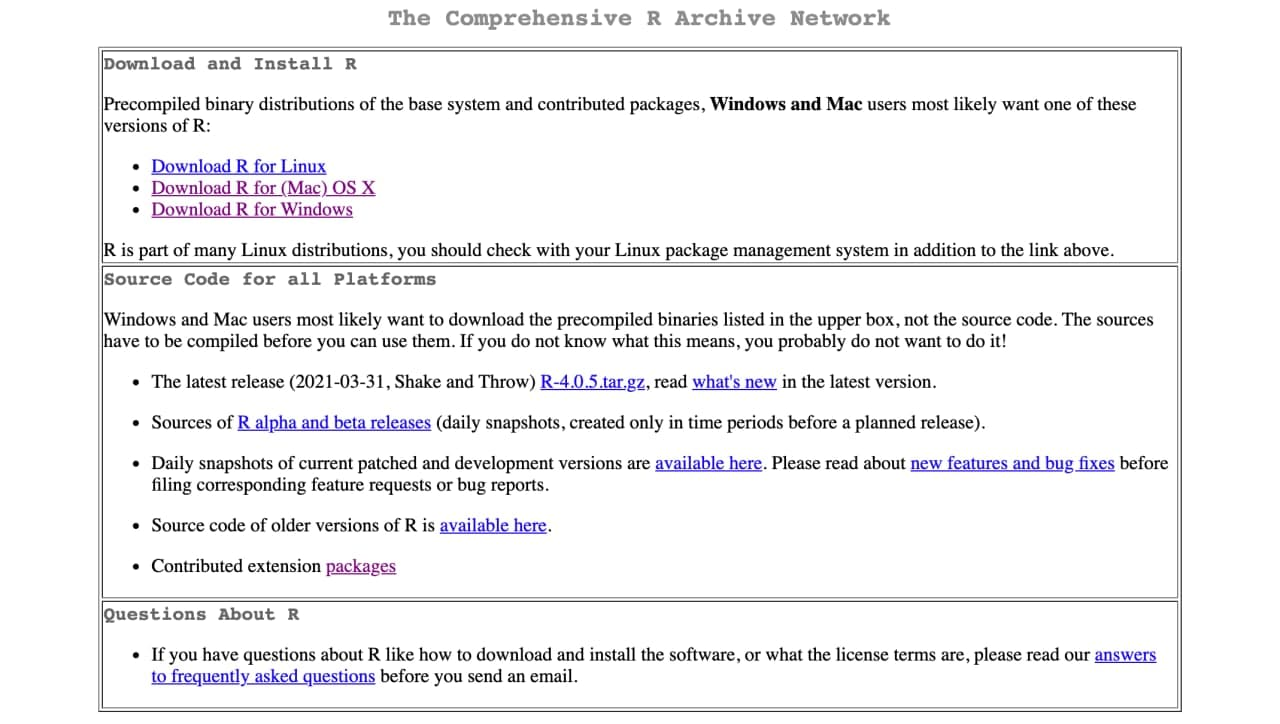
\includegraphics[width=0.8\linewidth]{./img/pantalla1_cran} 

}

\caption{Pantalla inicial de la plataforma CRAN de R.}\label{fig:pantalla-cran}
\end{figure}

\begin{itemize}
\tightlist
\item
  \textbf{Paso 2}: para sistemas operativos \textbf{Mac} basta con que hacer click en el archivo \texttt{.pkg}, y abrirlo una vez descargado (ver imagen \ref{fig:pantalla-mac})
\end{itemize}

\begin{figure}

{\centering 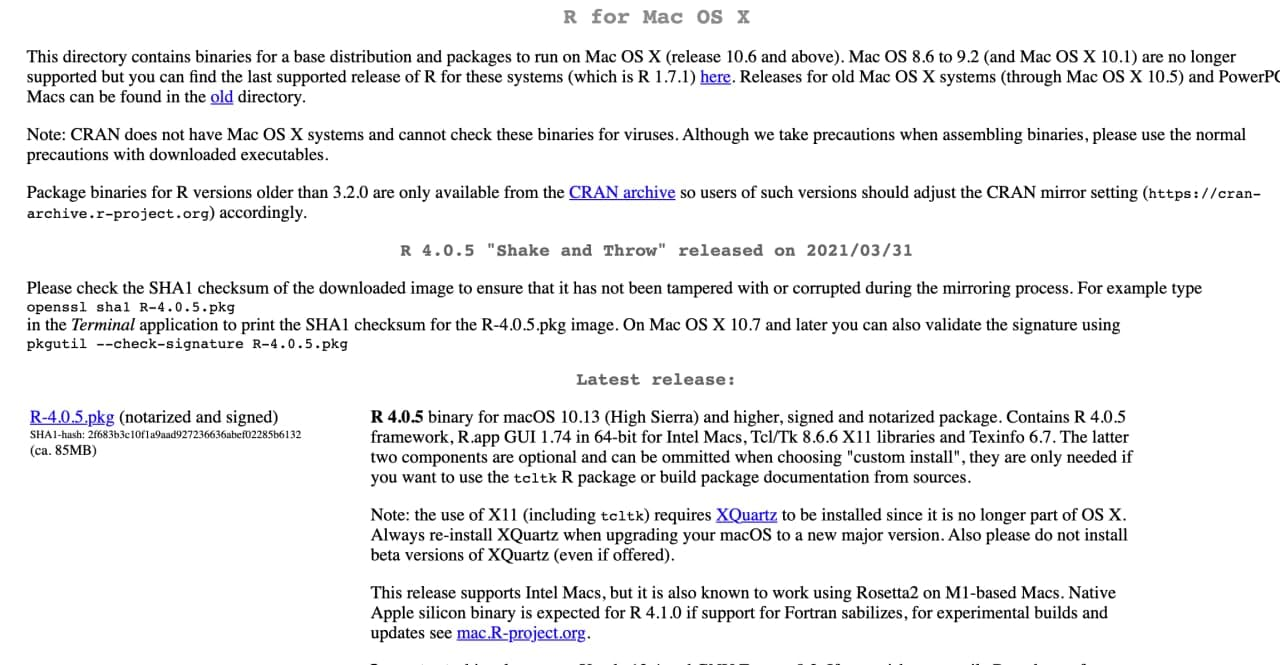
\includegraphics[width=0.9\linewidth]{./img/pantall_mac_cran} 

}

\caption{Pantalla de instalación de R en Mac OS.}\label{fig:pantalla-mac}
\end{figure}

Para sistemas operativos \textbf{Windows}, debemos clickar en \texttt{install\ R\ for\ the\ first\ time} (ver imagen \ref{fig:pantalla-windows-1}) y en la siguiente pantalla hacer click en \texttt{Download\ R\ for\ Windows} (ver imagen \ref{fig:pantalla-windows-2}). Una vez descargado, abrirlo como cualquier archivo de instalación.

\begin{figure}

{\centering 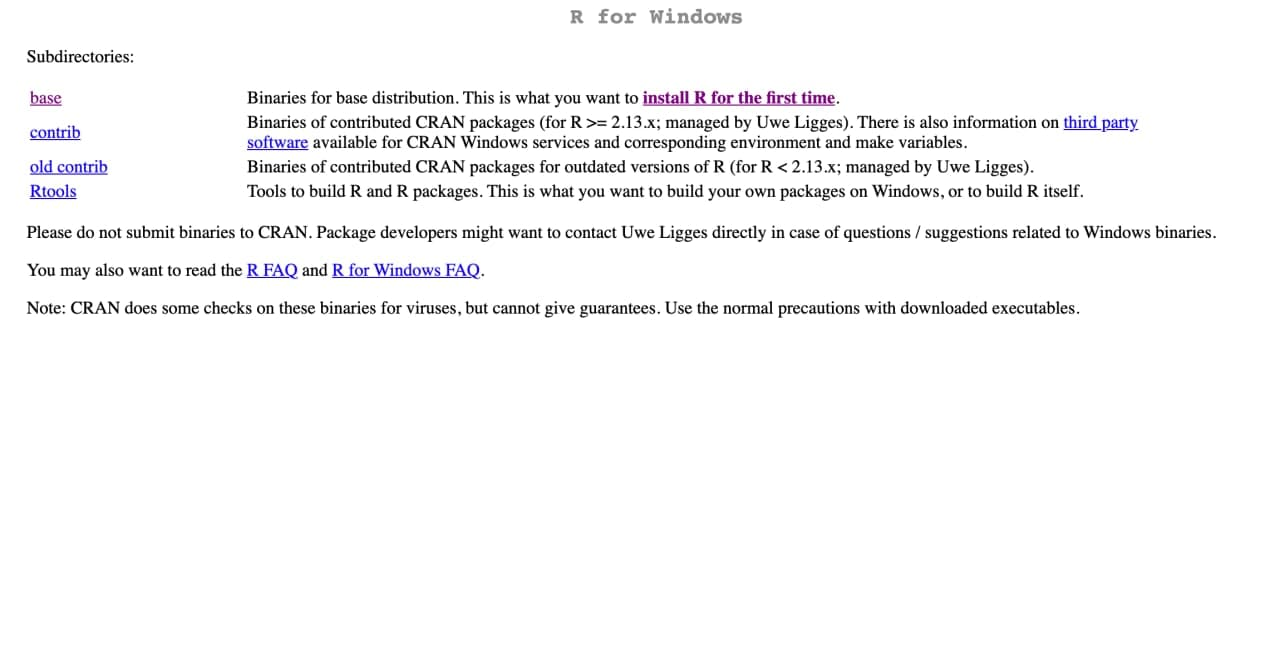
\includegraphics[width=0.8\linewidth]{./img/pantalla_windows_1} 

}

\caption{Pantalla previa de instalación de R en Windows.}\label{fig:pantalla-windows-1}
\end{figure}

\begin{figure}

{\centering 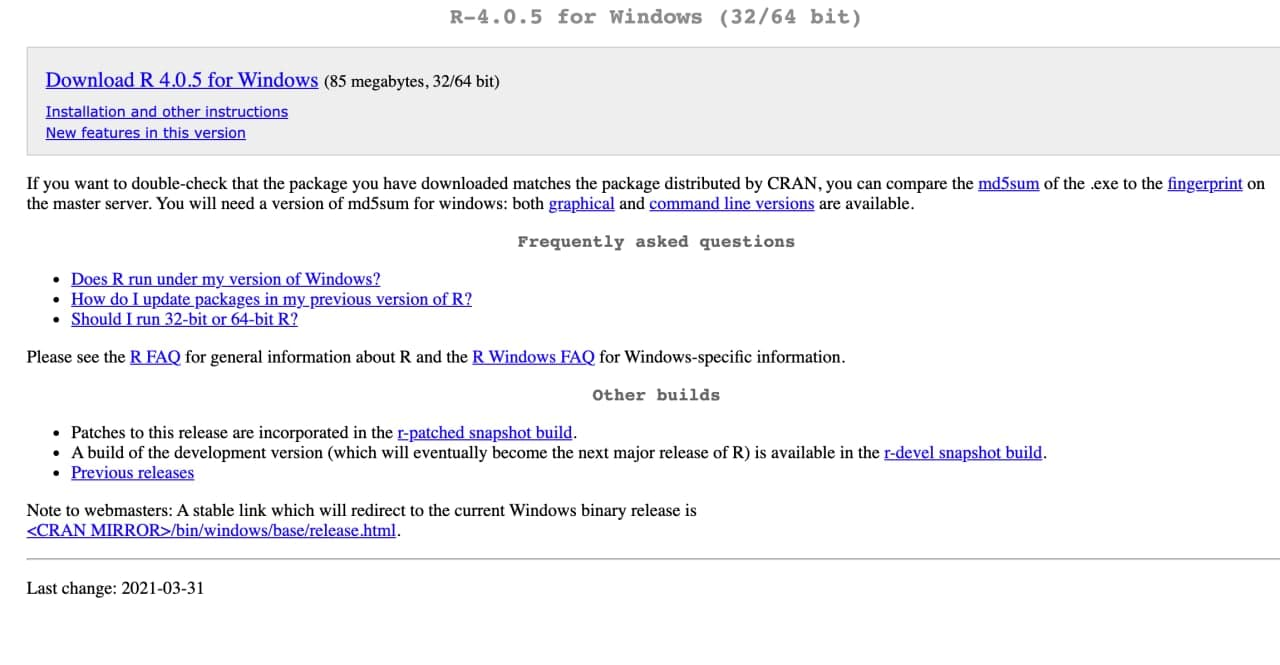
\includegraphics[width=0.9\linewidth]{./img/pantalla_windows_2} 

}

\caption{Pantalla final de instalación de R en Windows.}\label{fig:pantalla-windows-2}
\end{figure}

\begin{itemize}
\tightlist
\item
  \textbf{Paso 3}: tras su instalación tendrás en tu escritorio (Windows) o en tu Launchpad (Mac Os) un \textbf{ejecutable de \texttt{R} para abrir}. En Windows puede que tengas dos ejecutables \texttt{i386} y \texttt{x64} (como todo programa en Windows, está la versión de 32 y de 64 bits, haz click preferiblemente - si lo tienes - en el de \texttt{x64}). Te saldrá algo parecido a lo que observas en la imagen \ref{fig:cranR}.
\end{itemize}

\begin{figure}

{\centering 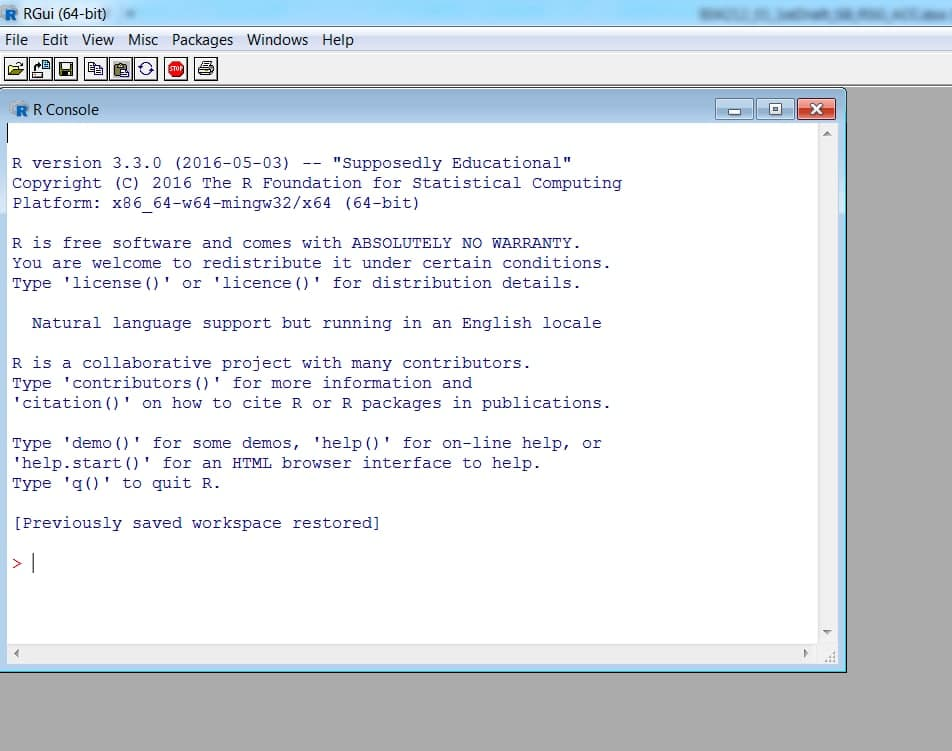
\includegraphics[width=0.75\linewidth]{./img/cranR} 

}

\caption{Primera pantalla al abrir el ejecutable de R.}\label{fig:cranR}
\end{figure}

\hypertarget{primera-operaciuxf3n-sumar-dos-nuxfameros}{%
\subsection{Primera operación: sumar dos números}\label{primera-operaciuxf3n-sumar-dos-nuxfameros}}

Para comprobar que está correctamente instalado, abre \texttt{R} y \textbf{prueba a escribir} en la pantalla blanca inferior el siguiente código (\textbf{recuerda}: los códigos de este manual puedes \textbf{copiarlos} directamente de la cajita \textbf{haciendo click en el botón} de la esquina superior derecha)

\begin{Shaded}
\begin{Highlighting}[]
\NormalTok{a <-}\StringTok{ }\DecValTok{1}
\NormalTok{b <-}\StringTok{ }\DecValTok{2}
\NormalTok{a }\OperatorTok{+}\StringTok{ }\NormalTok{b}
\end{Highlighting}
\end{Shaded}

\begin{verbatim}
## [1] 3
\end{verbatim}

\begin{figure}

{\centering 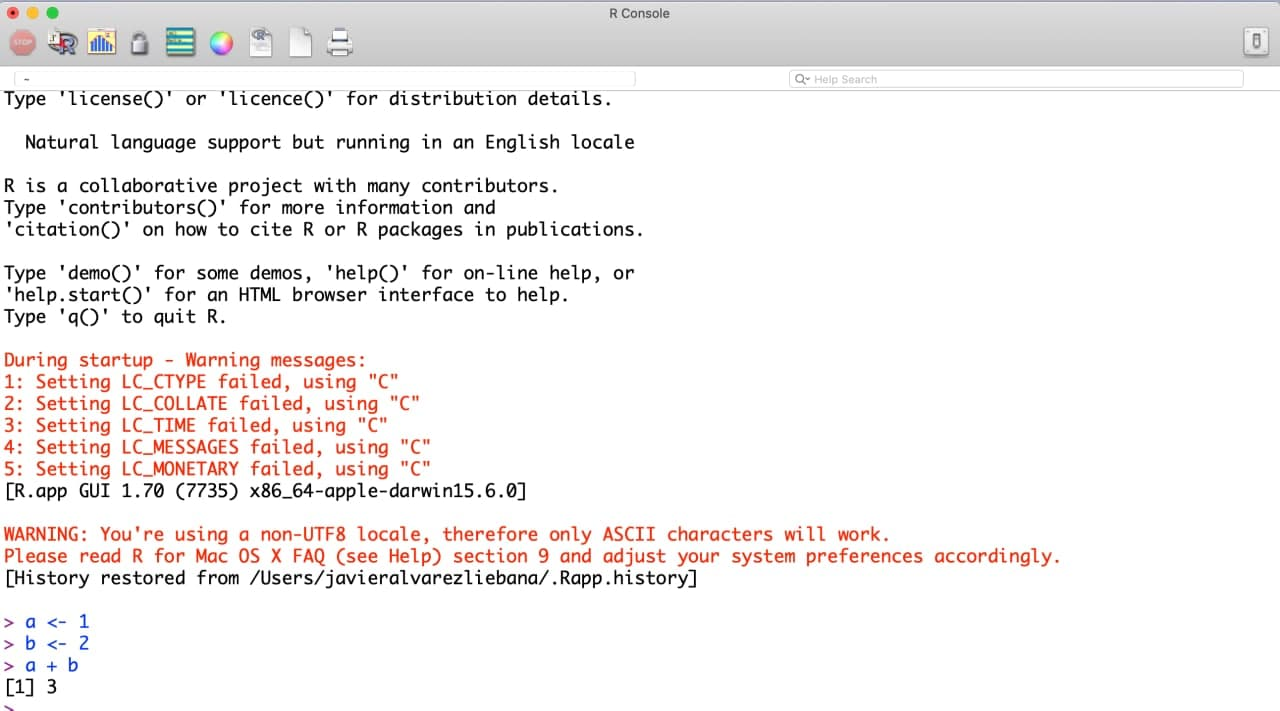
\includegraphics[width=0.9\linewidth]{./img/primera_suma} 

}

\caption{Primera suma en la consola de R.}\label{fig:primera-suma}
\end{figure}

\textbf{¡Enhorabuena!}

\begin{itemize}
\item
  \textbf{¿Dónde hemos escrito ese código?} Esa pantalla blanca donde hemos escrito el código se llama \textbf{CONSOLA}, y será donde ejecutaremos las órdenes.
\item
  \textbf{¿Qué hemos hecho?} Hemos hecho más de lo que parece. Primero, hemos definido dos variables \texttt{a} y \texttt{b} \textbf{asignándole un valor numérico a cada una de ellas}. Imagina que el símbolo \texttt{\textless{}-} es visto en nuestra cabeza como una flecha: a una variable que llamamos \texttt{a} le asignamos el valor \texttt{1}, a una variable que llamamos \texttt{b} le asignamos el valor \texttt{2}. Podemos verlo como \(a = 1,~b = 2\). Y tras definir dichas variables, las hemos usado en una \textbf{operación aritmética} \texttt{a\ +\ b}. Ya sabemos usar \texttt{R} como \textbf{calculadora}.
\item
  \textbf{¿Cómo nos devuelve \texttt{R} el resultado de la operación?} Si te ha devuelto el resultado correcta, en la consola debe aparecer \texttt{{[}1{]}\ 3}. El valor \texttt{{[}1{]}} aparecerá siempre ya que simplemente nos \textbf{numera las líneas} de la consola usadas; lo que viene detrás es realmente el resultado, es decir, \(a + b = 3\).
\item
  \textbf{¿Por qué hemos escrito \texttt{a\ +\ b} al final?} Un mantra de \texttt{R}, que veremos a lo largo de todo el curso, es que \textbf{\texttt{R} intenta molestarte lo menos posible} (eso es bueno cuando ya sabes usarlo, no tan bueno cuando empezamos a aprenderlo). Cuando asignamos los valores \texttt{a\ \textless{}-\ 1} y \texttt{b\ \textless{}-\ 2}, \texttt{R} no nos muestra nada: si guardamos un resultado en una variable, no nos muestra nada por consola. Para obtener el resultado en la consola necesitamos escribir el nombre de las variables (u operaciones entre ellas, como \texttt{a\ +\ b}).
\end{itemize}

~

\textbf{\textcolor{#ffc107}{WARNING: }}

Como habrás advertido, en \texttt{R} usaremos \texttt{\textless{}-} para \textbf{asignar valores} en lugar de \texttt{=}, como una flecha. Usaremos \texttt{=} para \textbf{\textcolor{#ffc107}{indicarle el valor a los argumentos que usemos en funciones}} y \texttt{==} como \textbf{\textcolor{#ffc107}{operador de comparación}}: si escribimos \texttt{2\ ==\ 3}, le estamos preguntando si 2 es igual a 3.

\begin{Shaded}
\begin{Highlighting}[]
\DecValTok{2} \OperatorTok{==}\StringTok{ }\DecValTok{3}
\end{Highlighting}
\end{Shaded}

\begin{verbatim}
## [1] FALSE
\end{verbatim}

~

Bonita esta interfaz no es, así que la cerraremos y no la abriremos más. Tenemos nuestro lenguaje instalado, vamos a \textbf{instalar nuestro Word} para poder programar de forma cómoda.

\hypertarget{instalacionRStudio}{%
\section{Instalación de R Studio}\label{instalacionRStudio}}

Para instalar \texttt{RStudio} deberemos ir a la web \url{https://www.rstudio.com/products/rstudio/download/\#download} (el gratuito) y seleccionar el ejecutable que te aparezca acorde a tu sistema operativo (ver imagen \ref{fig:pantalla-rstudio}). Tras descargar el ejecutable, hay que abrirlo como otro cualquier otro ejecutable y dejar que termine la instalación.

\begin{figure}

{\centering 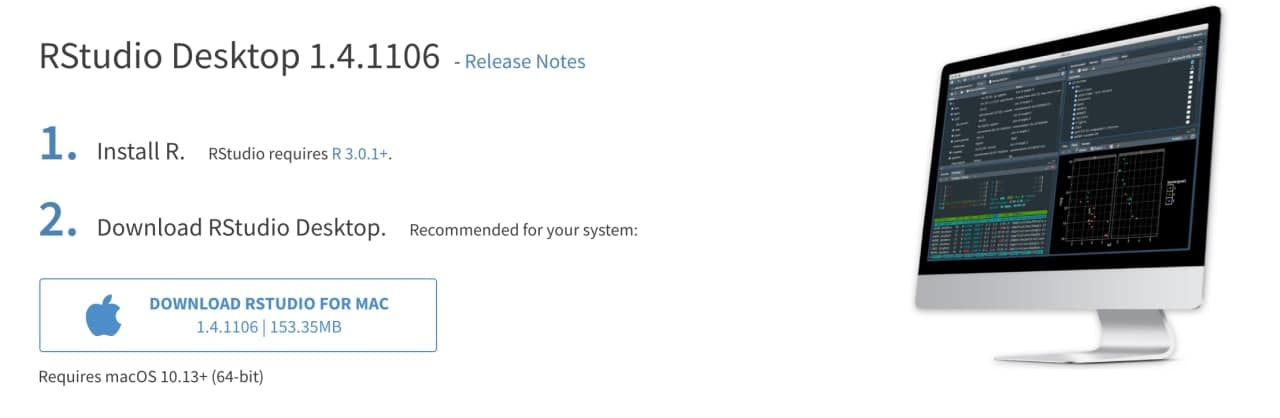
\includegraphics[width=0.7\linewidth]{./img/pantalla_rstudio} 

}

\caption{Descargar el ejecutable de RStudio para su posterior instalación.}\label{fig:pantalla-rstudio}
\end{figure}

Tras instalar tendremos en el escritorio o Launchpad un ejecutable de \texttt{RStudio} que abriremos. Se nos aparecerá una pantalla similar a esta:

\begin{figure}

{\centering 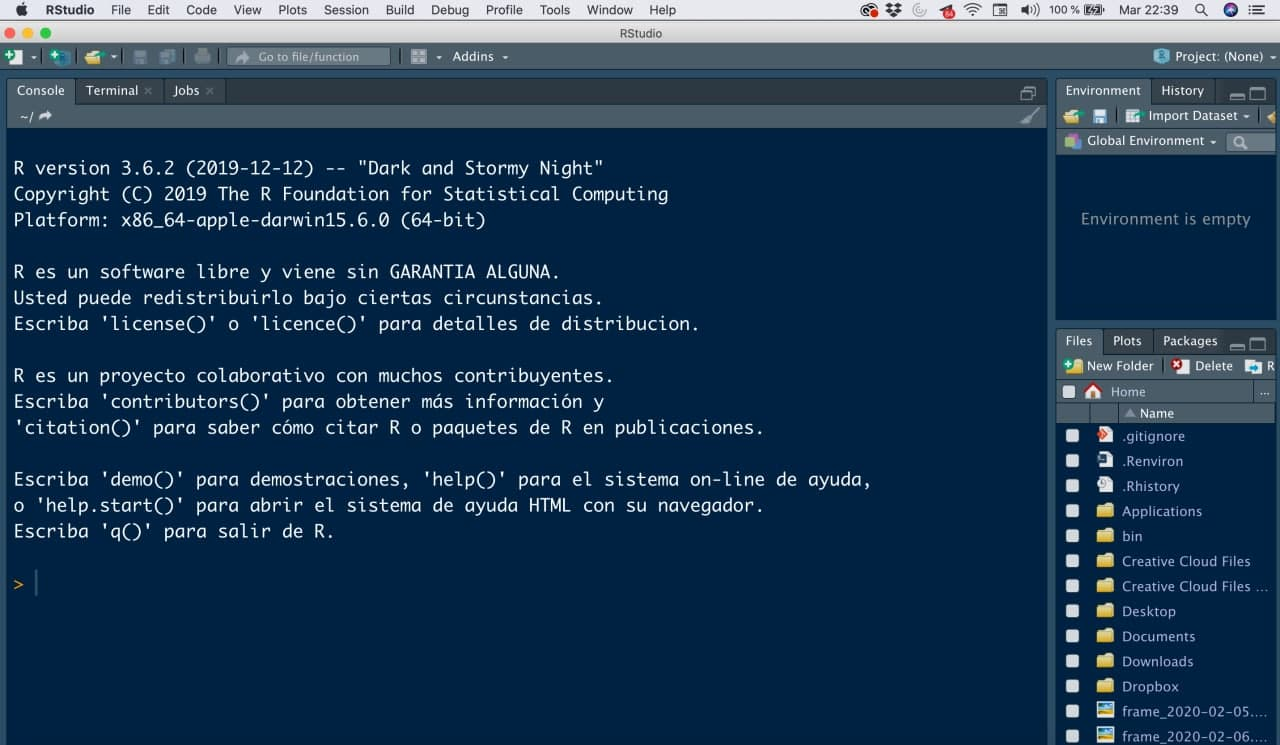
\includegraphics[width=0.85\linewidth]{./img/inicio_rstudio_1} 

}

\caption{Primer recibimiento de nuestro mejor amigo RStudio.}\label{fig:inicio-rstudio-1}
\end{figure}

Listo, tienes \textbf{instalado (casi) todo} correctamente.

\hypertarget{glosario}{%
\section{Glosario}\label{glosario}}

\textbf{\textcolor{#4197D2}{GLOSARIO}}

\begin{itemize}
\tightlist
\item
  \textbf{\textcolor{#4197D2}{Consola}}: es el nombre para llamar a esa ventana grande que te ocupa buena parte de tu pantalla. Prueba a escribir el mismo código que antes en ella (es el equivalente a la consola de R que hemos abierto al principio).
\end{itemize}

\begin{Shaded}
\begin{Highlighting}[]
\NormalTok{a <-}\StringTok{ }\DecValTok{1}
\NormalTok{b <-}\StringTok{ }\DecValTok{2}
\NormalTok{a }\OperatorTok{+}\StringTok{ }\NormalTok{b}
\end{Highlighting}
\end{Shaded}

\begin{figure}

{\centering 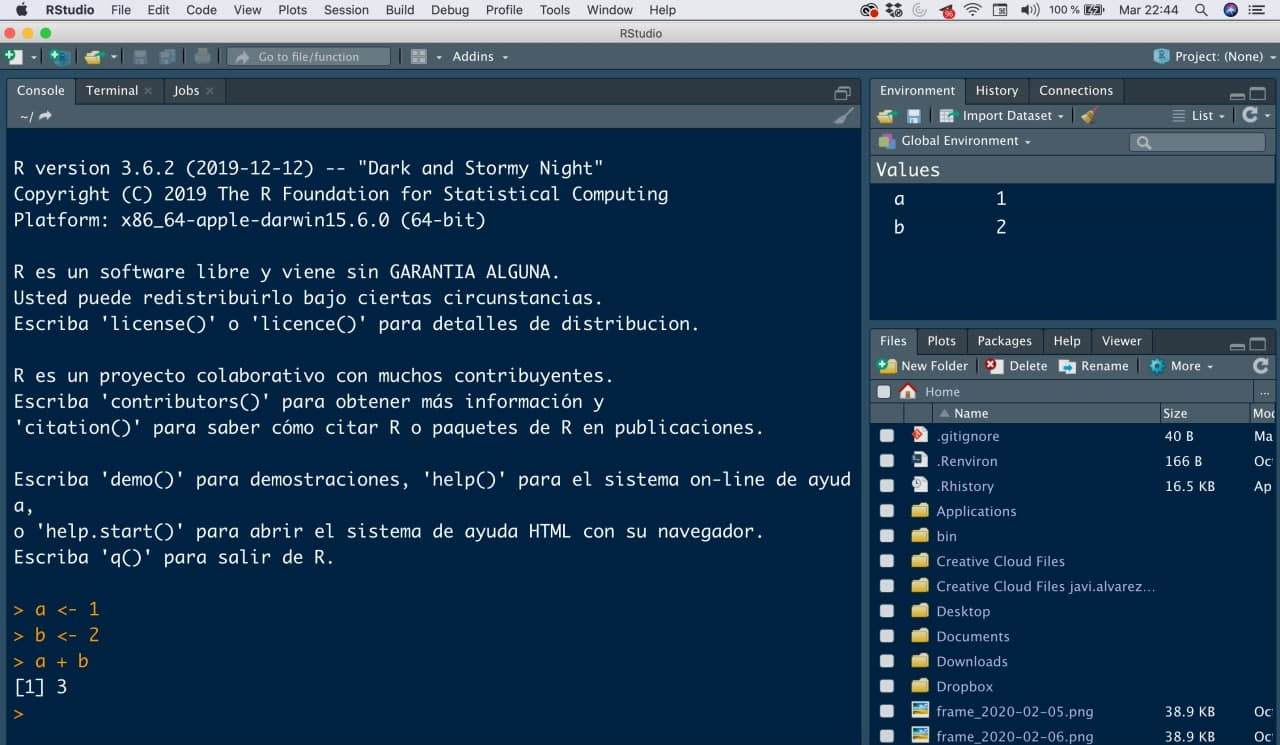
\includegraphics[width=0.6\linewidth]{./img/inicio_rstudio_2} 

}

\caption{Lanzando a consola nuestras primeras órdenes en RStudio.}\label{fig:inicio-rstudio-2}
\end{figure}

\textbf{\textcolor{#4197D2}{La consola será donde ejecutaremos órdenes y mostraremos resultados}}

\begin{itemize}
\tightlist
\item
  \textbf{\textcolor{#4197D2}{Environment (entorno)}}: la pantalla pequeña (puedes ajustar los márgenes con el ratón a tu gusto) que tenemos en la parte superior derecha se denomina environment o entorno de variables, donde como puedes ver, tras ejecutar el pequeño código en la consola, nos informa de que tenemos dos variables numéricas y su valor asignado. Nos \textbf{mostrará las variables que tenemos definidas, el tipo y su valor}.
\end{itemize}

\begin{figure}

{\centering 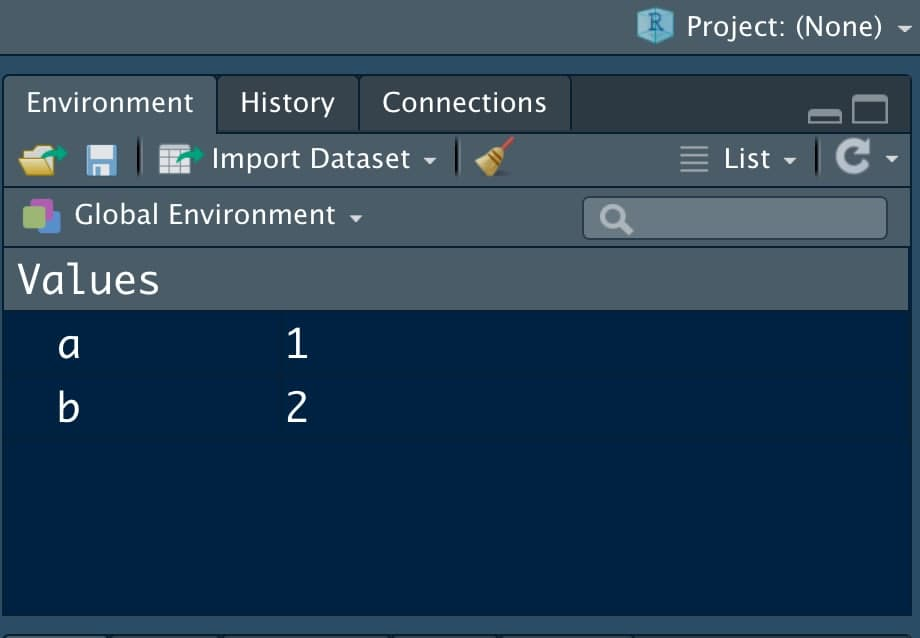
\includegraphics[width=0.65\linewidth]{./img/inicio_rstudio_3} 

}

\caption{Environment de variables.}\label{fig:inicio-rstudio-3}
\end{figure}

\begin{itemize}
\tightlist
\item
  \textbf{\textcolor{#4197D2}{Panel multiusos}}: la ventana que tenemos en la parte inferior derecha no servirá para buscar ayuda de comandos y órdenes, además de para visualizar gráficos. Lo veremos cuando sea necesario.
\end{itemize}

\begin{figure}

{\centering 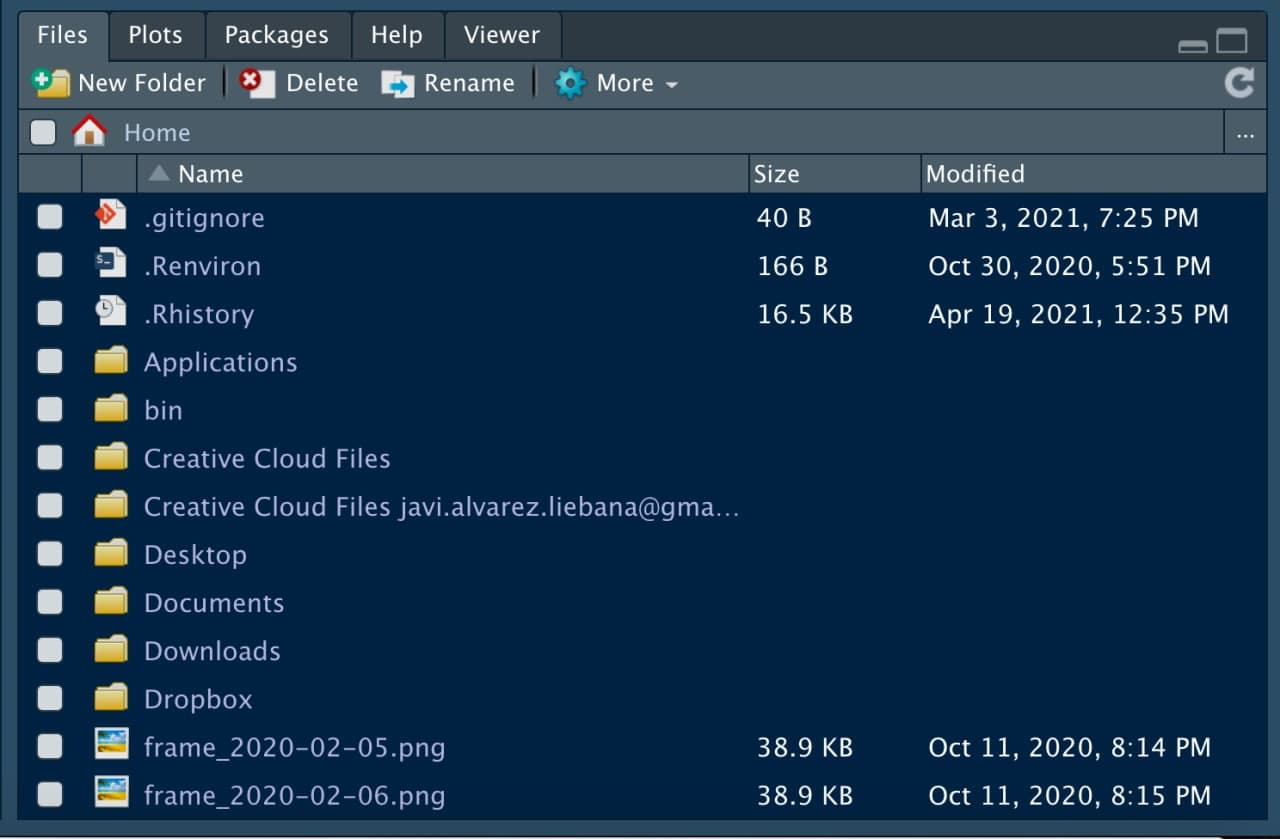
\includegraphics[width=0.65\linewidth]{./img/inicio_rstudio_4} 

}

\caption{Panel multiusos.}\label{fig:inicio-rstudio-4}
\end{figure}

\hypertarget{consejos}{%
\section{Consejos}\label{consejos}}

\textbf{\textcolor{#20935E}{CONSEJOS}}

\textbf{\textcolor{#20935E}{¿Cómo saber cuando la orden lanzada en consola ha terminado?}}

A veces \texttt{R} y \texttt{RStudio} son tan silenciosos que no sabemos si ha acabado la orden que acabamos de lanzar en la consola o no. Siempre que veas el símbolo \texttt{\textgreater{}} como última línea en la consola significa que está listo para que le escribamos otra orden (es la forma cariñosa de decirte que ya ha acabado, ver imagen \ref{fig:tip-consola-lista})

\begin{figure}

{\centering 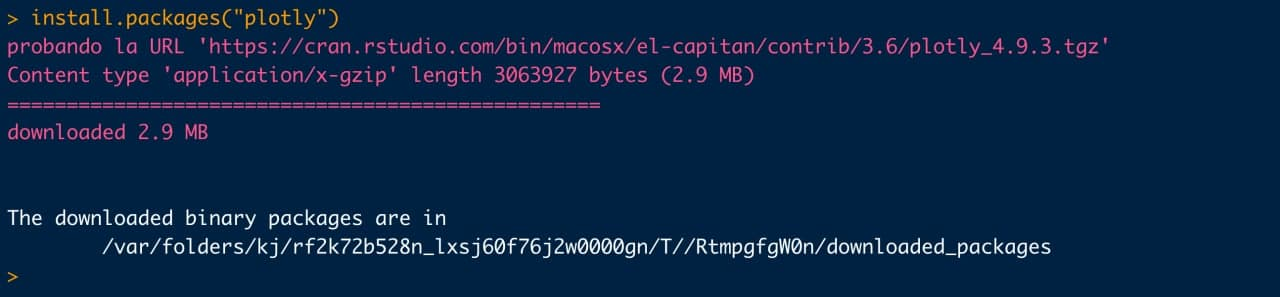
\includegraphics[width=0.7\linewidth]{./img/tip_consola_lista} 

}

\caption{Ejemplo de que la orden lanzada ha acabado.}\label{fig:tip-consola-lista}
\end{figure}

~

\textbf{\textcolor{#20935E}{¿Cómo prevenir la fatiga programando?}}

Estando delante de una pantalla de ordenador, con la vista muy fija mientras se programa, puede que acabes teniendo cierta fatiga visual en el trabajo. Te aconsejo que cambies en tu \texttt{RStudio} la tonalidad del fondo de tu programa, en tonos oscuros y no blancos (¿te has fijado que mis capturas tienen un azul cobalto oscuro de fondo mientras el tuyo es un \textbf{blanco nuclear}? Echa un vistazo a las imágenes \ref{fig:menu-1} y \ref{fig:menu-2})

\begin{figure}

{\centering 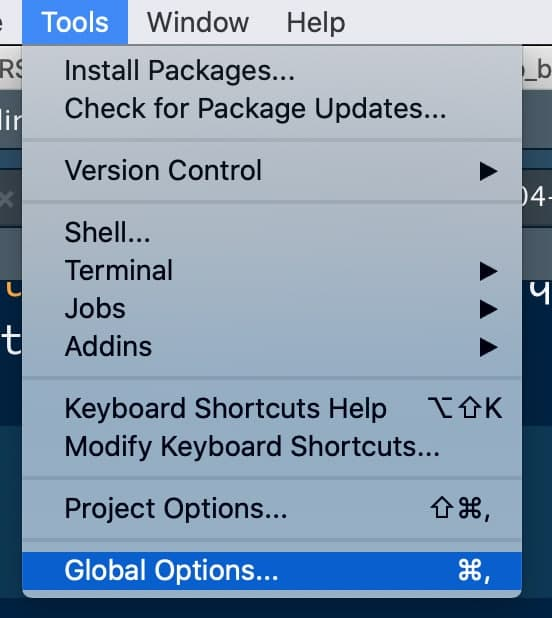
\includegraphics[width=0.5\linewidth,height=0.5\textheight]{./img/menu_1} 

}

\caption{Menú de opciones de nuestro editor}\label{fig:menu-1}
\end{figure}

\begin{figure}

{\centering 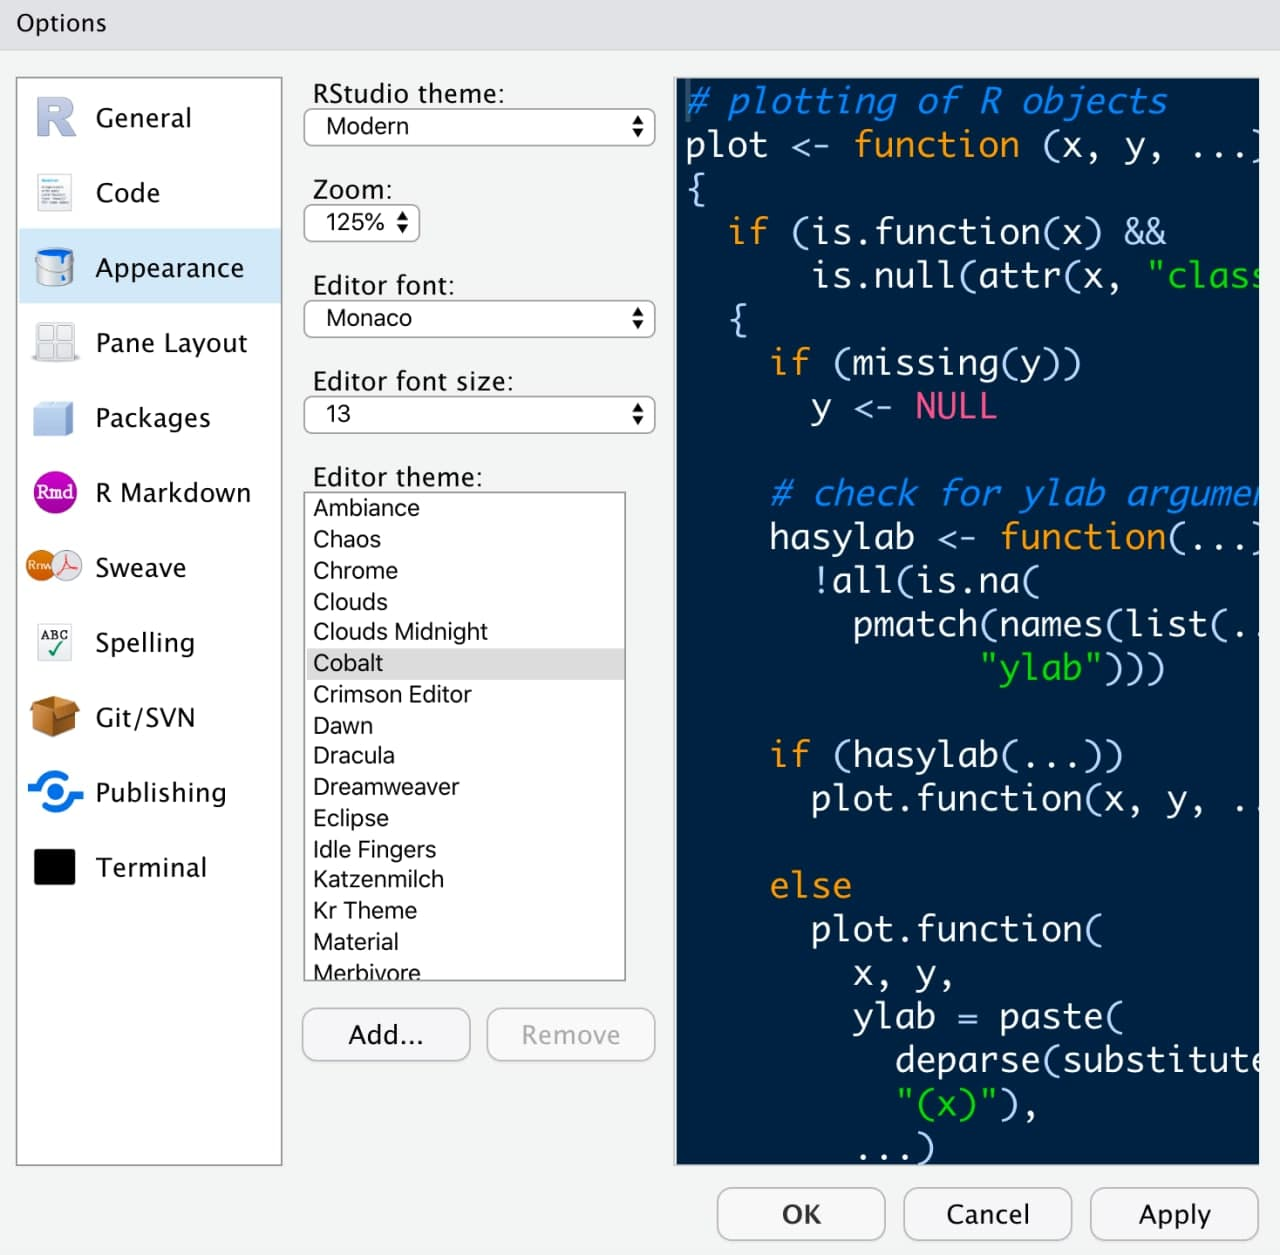
\includegraphics[width=0.5\linewidth,height=0.5\textheight]{./img/menu_2} 

}

\caption{Personalizar el color de fondo de nuestro editor, la letra y el tamaño de fuente}\label{fig:menu-2}
\end{figure}

\hypertarget{que-es-R}{%
\chapter{¿Qué es R?}\label{que-es-R}}

Una vez que tenemos todo instalado vamos a dar nuestros \textbf{primeros pasos} en \texttt{R}, pero antes veamos un poco de su historia y de una particularidad: \texttt{R} es un \textbf{lenguaje modular} (¿modu\ldots{}qué?)

\hypertarget{historia-de-r}{%
\section{Historia de R}\label{historia-de-r}}

Veamos antes un poco de la \textbf{historia} de nuestra deidad.

Allá por 1975, los \textbf{laboratorios Bell} (los que inventaron la radio moderna tal y como la conocemos), necesitaban una alternativa a los lenguajes más «rudos» y antiguos como \texttt{C++} o \texttt{Fortran}, lenguajes rápidos en la ejecución pero complejos en su uso, con una gran curva de aprendizaje y con \textbf{muy poca capacidad en la visualización de datos} que se empezaba a necesitar.

Así que en \textbf{1976 sacaron la primera versión del lenguaje conocido \texttt{S}} (hasta entonces estaba de moda lo de llamar a los lenguajes con una sola inicial). En \textbf{1980} se empezó a distribuir la primera versión pública de \texttt{S}, más allá de los laboratorios Bell, y en \textbf{1988} se añadieron bastantes funcionalidades nuevas como poder aplicar funciones a otras funciones (los famosos \texttt{apply()} que ya veremos). Años más tarde, en \textbf{1991}, dicho lenguaje se simplificó, reescribiendo muchas subrutinas de otros lenguajes más primitivos, para tener una versión muy parecida al actual \texttt{R}, permitiendo el usod de operadores, \texttt{data.frames} (que veremos) y otro tipo de objetos, sencillos en la programación pero muy versatiles.

Sin embargo, salvo uso docente, \texttt{S} tenía licencia así que \textbf{en 1992 Ross Ihaka y Robert Gentleman se lanzaron a crear una versión de \texttt{S} libre y gratuita}, un trabajo de casi 8 años hasta que en el año 2000, ambos investigadores de la Universidad de Auckland en Nueva Zelanda lanzaron la primera versión estable del lenguaje.

Tras dicho lanzamiento, se creó un \textbf{equipo de expertos en estadística computacional} (el conocido como \emph{R Development Core Team}) que es el que se encarga de mantener toda la aerquitectura de \texttt{R} y los que se encargar de actualizar y mejorar el paquete \texttt{\{base\}}, una \textbf{librería motor} sobre la que se construye el resto de funciones.

Y es precisamente ese hecho una de las principales diferencias entre \texttt{Python} y \texttt{R}: \texttt{R} fue creado por y para estadísticos. Te dejo esta \href{https://dadosdelaplace.github.io/202112_R-python/}{entrada en el blog} por si quieres curiosear las diferencias (aunque ambos pueden ser útiles para trabajos estadísticos muy generales).

\hypertarget{instalacionpaquetes}{%
\section{Comunidad de usuarios: paquetes}\label{instalacionpaquetes}}

La pregunta del millón suele ser siempre la misma: \textbf{¿qué lenguaje elegir?} Podríamos hacer una comparativa técnico de distintos lenguajes pero vamos a quedarnos con dos \textbf{consejos fundamentales}: prioriza el software libre y aquellos lenguajes que tienen una \textbf{comunidad muy grande de usuarios} trabajando en los problemas o campo para el que vas a usar dicho lenguaje.

El lenguaje \texttt{R} (también \texttt{Python}) tiene \textbf{3 ventajas principales}:

\begin{itemize}
\item
  Es un \textbf{lenguaje creado por y para estadísticos/as}.
\item
  Es \textbf{software libre} (como C++, Python, Fortran, y otros tantos lenguajes). El software libre no solo tiene una ventaja evidente (es gratis, ok) sino que permite acceder libremente a código ajeno.
\item
  Es un \textbf{lenguaje modular}: en la instalación que hemos realizado no se han instalado todas las funcionalidades, solo el mínimo para poder funcionar, de forma que se ahorra espacio en disco y en memoria. Al ser software libre, existen trozos de código hechos por otras personas llamados \textbf{paquetes}, que podemos ir instalando a nuestro gusto según los vayamos necesitando. Esto es una ventaja enorme ya que \texttt{R} tiene una comunidad de usuarios gigante para hacer estadística (\texttt{Python} tiene una enorme comunidad pero más enfocada al \emph{Machine Learning}), con \textbf{más de 17 000 paquetes}: ¡hay más de 17 000 trozos de código, muchos de ellos programados por expertos/as en \texttt{R}, validados por la comunidad y la plataforma, y de forma gratuita!
\end{itemize}

\begin{figure}

{\centering 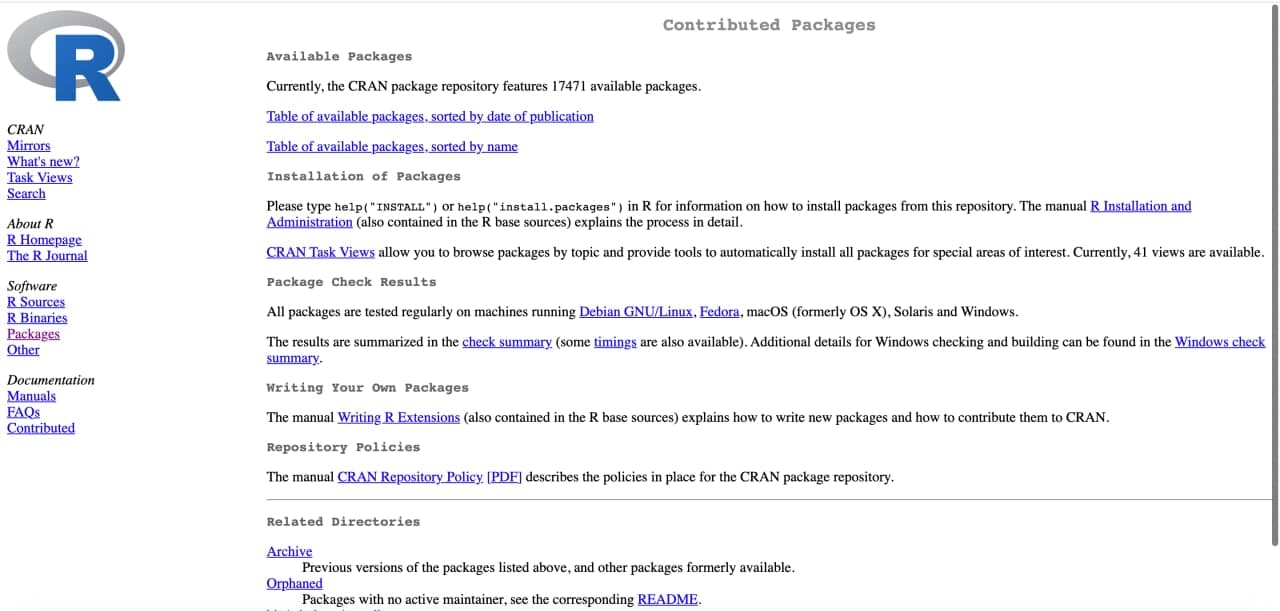
\includegraphics[width=0.7\linewidth]{./img/paquetes_R} 

}

\caption{Paquetes disponibles en R.}\label{fig:paquetes-R}
\end{figure}

Esto nos ahorra muchísimo tiempo en nuestro día a día ya que \textbf{casi todo lo que querramos hacer ya lo habrá querido hacer otra persona} (y seguramente mejor que nosotros/as). Vamos a instalar, por ejemplo, un paquete gráfico (\texttt{\{ggplot2\}}) que necesitaremos en el futuro. Para ello, escribe en tu consola el siguiente código y pulsa \emph{enter}.

\begin{Shaded}
\begin{Highlighting}[]
\KeywordTok{install.packages}\NormalTok{(}\StringTok{"ggplot2"}\NormalTok{)}
\end{Highlighting}
\end{Shaded}

Dicha orden (puede tardar un poco la primera vez, depende de tu conexión a internet) lo que hará será \textbf{acceder a la web de R}, \textbf{bajarse a tu ordenador los trozos de código} incluidos en el paquete llamado \texttt{\{ggplot2\}}, y dejarlos para siempre en él.

~

\textbf{\textcolor{#ffc107}{WARNING:}}

La \textbf{instalación de paquetes SOLO ES NECESARIA la primera vez} que se usa dicho paquete en la vida del ordenador, no hace falta hacerlo cada vez que lo usas.

~

Una vez que tenemos los trozos de código (el paquete) en nuestro ordenador, en cada sesión de \texttt{R} que abramos (cada vez que cierres y abras \texttt{RStudio}) deberemos (si queremos) llamar a ese paquete que tenemos instalado, escribiendo el siguiente comando en consola

\begin{Shaded}
\begin{Highlighting}[]
\KeywordTok{library}\NormalTok{(ggplot2)}
\end{Highlighting}
\end{Shaded}

\textbf{Welcome to software libre}

\hypertarget{por-quuxe9-excel-no-es-tu-amigo}{%
\section{¿Por qué Excel no es tu amigo?}\label{por-quuxe9-excel-no-es-tu-amigo}}

\textbf{\texttt{R} es un lenguaje de programación}, de alto nivel para el usuario y modular. Los lenguajes de alto nivel como \texttt{R}, \texttt{Python} (curso interactivo de Python en \url{https://checkio.org/}) o \texttt{Matlab}, facilitan la programación al usuario, teniendo que preocuparte solo de la tarea de programar. Son lenguajes con una \textbf{menor curva de aprendizaje} aunque suelen ser más lentos en su ejecución en comparación con lenguajes de bajo nivel (\texttt{C}, \texttt{C++} o \texttt{Fortran}), lenguajes muy rápidos en su ejecución pero cuya programación requiere un mayor tiempo y formación, teniendo que además estar pendiente del tipo de variables, espacio en memoria, etc.

Por su arquitectura, \texttt{R} es un lenguaje que puede ser usado para un propósito general pero que está especialmente diseñado para el \textbf{análisis estadístico de datos}. Su \textbf{modularidad} nos da la ventaja de que podemos instalar las funcionalidades que vayamos necesitando de forma progresiva.

\textbf{\textcolor{#20935E}{¿Por qué no es recomendable usar Excel como base de datos ni para realizar análisis estadísticos complejos?}}

~

\begin{itemize}
\item
  \textbf{Software de pago}: Excel, al igual que el resto de programas de Microsoft o SPSS (por desgracia programa estrella de nuestro sistema sanitario), es un programa de pago. A nivel individual, todos hemos tenido una versión que no hemos pagado, pero dicha evasión no se la puede permitir una empresa o administración, que debe de pagar altas cantidades de dinero anuales por las licencias, dinero que no sería necesario si los investigadores y trabajadores tuvieran formación (remunerada) en otras herramientas de software libre.
\item
  \textbf{Software cerrado}: no solo es de pago sino que es cerrado, así que solo podemos hacer lo que Excel ha creído que interesante que podamos hacer. Incluso con la programación de MACROS, las funcionalidades de Excel siguen siendo mucho más limitadas ya que viene «programadas» de antemano
\item
  \textbf{Alto consumo de memoria}: dicha programación predeterminada hace que Excel ocupe muchísimo espacio en el disco duro y tenga un alto consumo de memoria (la memoria es lo que te permite hacer varias tareas a la vez en tu ordenador).
\item
  \textbf{No es universal}: no solo es de pago sino que además, dependiendo de la versión que tengas de Excel, tendrá un formato distinto para datos como fechas, teniendo incluso extensiones distintas, de forma que un archivo \texttt{.xls} abierto por un Excel moderno puede provocar errores en la carga.
\item
  \textbf{¡ES SOLO UNA HOJA DE CÁLCULO!}: el propio Microsoft desaconseja el uso de Excel para el análisis de grandes volúmenes de datos. El Excel es una herramienta maravillosa para ser usada como una sencilla hoja de cálculo: llevar las cuentas de tu familia, de tu pequeño negocio, una declaración de la Renta sencilla, planificar viajes, etc. Pero el programa \textbf{NO ESTÁ DISEÑADO} para ser una base de datos ni para análisis detallado, y muchos menos pensado para generar un entorno flexible para el análisis estadístico y la visualización de datos.
\end{itemize}

~

\textbf{¿Puedes ser el mejor partiendo un filete con una cuchara?} Seguramente puedas (en Excel puedes hasta programar con macros), y si siempre lo hiciste así, acabarás normalizándolo, pero seguirás siendo una persona comiendo filete con cuchara.

\textbf{¿Qué sucede si usamos la herramienta equivocada?} Tres ejemplos:

\begin{itemize}
\tightlist
\item
  \textbf{\textcolor{#dc3545}{Problemas para codificar fechas}}: en 2016 se publicó una \href{https://genomebiology.biomedcentral.com/articles/10.1186/s13059-016-1044-7}{revisión de artículos en genética}, descubriendo que 1 de cada 5 artículos contenían errores debido a una mala codificación de las fechas, conviertiendo por ejemplo los genes Septin-2 (conocido como SEPT2) en fechas, y al revés \citep{Ziemannetal16}.
\end{itemize}

\begin{figure}

{\centering 
\includegraphics[width=0.5\linewidth]{./img/excel_genes} 

}

\caption{Excel en una noche loca.}\label{fig:excel-genes}
\end{figure}

\begin{itemize}
\tightlist
\item
  \textbf{\textcolor{#dc3545}{Problemas de memoria}}: un Excel permite por defecto una cantidad máxima de filas. Aunque dicha cantidad se puede ampliar, sigue siendo finita, por lo que cuando superas el umbral de filas, al añadir filas Excel te borra registros \textbf{sin avisarte de que lo está haciendo}. Esto es lo que sucedió con los \href{https://www.redaccionmedica.com/secciones/sanidad-hoy/covid-reino-unido-pierden-16000-positivos-9989}{registros de casos covid en Reino Unido}.
\end{itemize}

\begin{figure}

{\centering 
\includegraphics[width=0.5\linewidth]{./img/excel_uk} 

}

\caption{Cuando Excel dice basta.}\label{fig:excel-uk}
\end{figure}

\begin{itemize}
\tightlist
\item
  \textbf{\textcolor{#dc3545}{Problemas para codificar edades}}: una variable de tipo fecha, aunque nosotros la veamos con letras, en realidad es una variable numérica que representa los días que han pasado desde una fecha origen. En función de las distintas versiones de Excel, dicha fecha origen cambia. Además, si se codifica mal la fecha en formato \texttt{dd-mm-YY}, dicho formato cuando se exporta a otro excel en texto, no permite distinguir a un nacido en 1918 y a un nacido en 2018, así que podemos estar confundiendo personas de 103 años con niños de 3 años (y es lo que \href{https://www.niusdiario.es/sociedad/sanidad/sanidad-reconoce-datos-muertes-ninos-covid-erroneos-contabilizaban-centenarios-como-menores_18_3107220241.html}{sucedió en España}, observando unas tasas de mortalidad en niños muy pequeños equivalentes a personas mayores).
\end{itemize}

\begin{figure}

{\centering 
\includegraphics[width=0.5\linewidth]{./img/excel_edades} 

}

\caption{Los centenarios con biberón.}\label{fig:excel-edades}
\end{figure}

\hypertarget{glosario-1}{%
\section{Glosario}\label{glosario-1}}

\textbf{\textcolor{#4197D2}{GLOSARIO}}

\begin{itemize}
\tightlist
\item
  \textbf{\textcolor{#4197D2}{Paquete}}: trozos de código realizadas por otros usuarios de la comunidad (y validades por el equipo de CRAN si la descarga es mediante \texttt{install.packages()}) para ser usados. Una vez instalados (descargados) los trozos de código a nuestro ordenador, basta con «acudir» a ellos con \texttt{library()}.
\end{itemize}

Haciendo una metáfora con la colección de libros que tengas en casa: con la \textbf{instalación hemos comprado el libro} y lo tenemos en nuestra estantería (para siempre), con la llamada al paquete, por ejemplo \texttt{library(ggplot2)}, lo que hacemos es decidir, de entre todos los libros de la estantería, cuales queremos llevarnos de viaje (en cada maleta que hagamos).

Los \textbf{paquetes usados} los verás denotados como \texttt{\{nombre\_paquete\}} a lo largo del manual.

\hypertarget{primeros-pasos}{%
\chapter{Primeros pasos}\label{primeros-pasos}}

\begin{blackbox}

Scripts usados:

\begin{itemize}
\tightlist
\item
  \href{https://github.com/dadosdelaplace/courses-ECI-2022/blob/main/scripts/script01.R}{\textbf{script01.R}}: ejercicio 4. Ver en \url{https://github.com/dadosdelaplace/courses-ECI-2022/blob/main/scripts/script01.R}
\end{itemize}


\end{blackbox}

~

Vamos a empezar por lo sencillo: \textbf{¿cómo usar \texttt{R} como una calculadora?}

\hypertarget{primeros-pasos-en-r-calculadora}{%
\section{Primeros pasos en R: calculadora}\label{primeros-pasos-en-r-calculadora}}

¿Te acuerdas de lo que era la \textbf{consola}? En el caso de \texttt{RStudio}, la consola será esa pequeña pantalla que tenemos en la parte inferior (la pestaña \emph{Console}). Vamos a trabajar de momento solo en esa ventana inferior.

\begin{figure}

{\centering 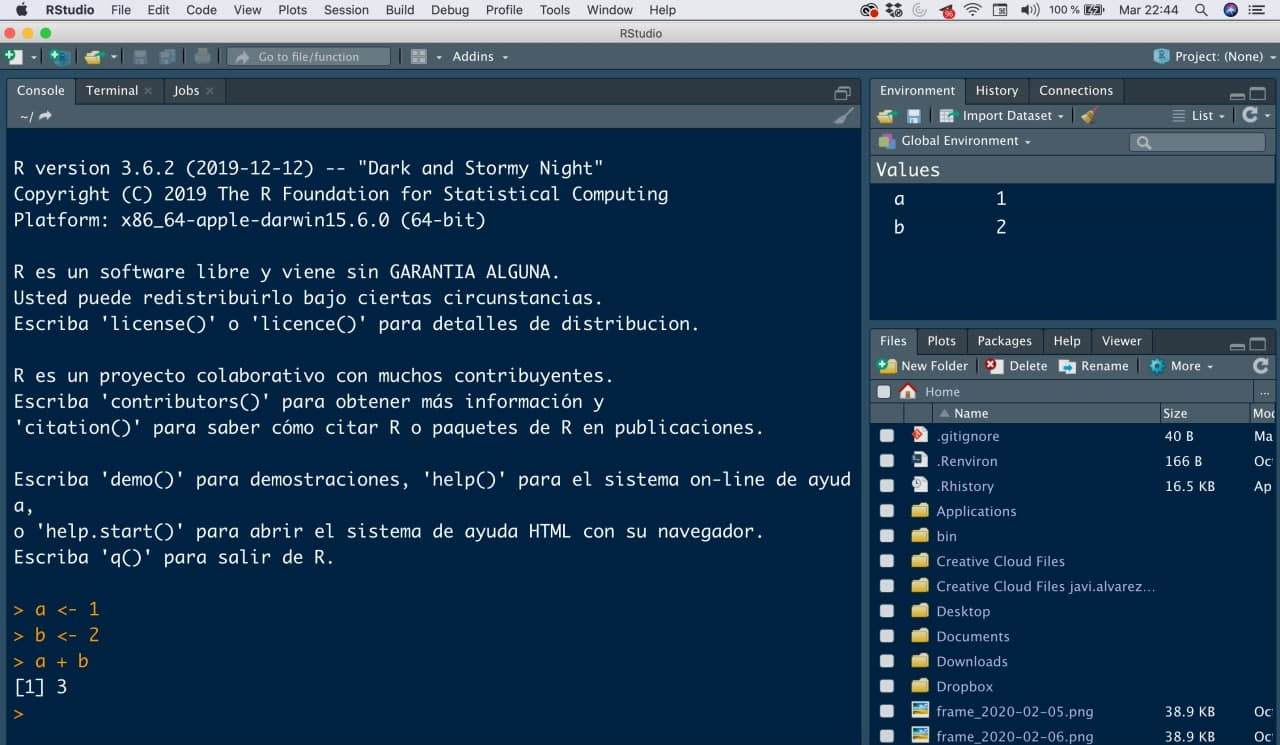
\includegraphics[width=0.75\linewidth]{./img/inicio_rstudio_2} 

}

\caption{Lanzando a consola nuestras primeras órdenes en RStudio.}\label{fig:inicio-rstudio-2a}
\end{figure}

Lo que ya hemos descubierto en los pasos de la instalación (ver imagen \ref{fig:inicio-rstudio-2a}) es que la consola de \texttt{R} tiene una función muy básica y evidente: nos sirve de calculadora. Un ejemplo muy simple: si escribimos 3 en la consola y pulsamos \emph{ENTER}, la consola nos mostrará el resultado de la suma

\begin{Shaded}
\begin{Highlighting}[]
\DecValTok{1} \OperatorTok{+}\StringTok{ }\DecValTok{2}
\end{Highlighting}
\end{Shaded}

\begin{verbatim}
## [1] 3
\end{verbatim}

~

\textbf{¿Cuál es la diferencia entre una calculadora y un lenguaje de programación?} Imagina que dicha suma 3 la quisiéramos utilizar para un segundo cálculo: ¿y si en lugar de lanzarlo a la consola sin más lo \textbf{almacenamos en alguna variable}?

Como hemos visto en la instalación de \texttt{RStudio}, para \textbf{asignar variables} lo haremos con \texttt{\textless{}-}, por ejemplo la orden \texttt{x\ \textless{}-\ 1\ +\ 2}: una variable de nombre \texttt{x} va a tener asignada lo que valga la suma \texttt{1\ +\ 2}

\begin{Shaded}
\begin{Highlighting}[]
\NormalTok{x <-}\StringTok{ }\DecValTok{1} \OperatorTok{+}\StringTok{ }\DecValTok{2}
\end{Highlighting}
\end{Shaded}

Como puedes comprobar, en tu parte superior derecha (nuestro \textbf{entorno de variables}), podrás ver como una nueva variable \texttt{x} es ahora visualizada, con su valor asignado (\textbf{no se mostrará en consola} salvo que escribas 3 en ella: \texttt{R} asume que no querías visualizarla en consola sino solo guardarla).

\begin{figure}

{\centering 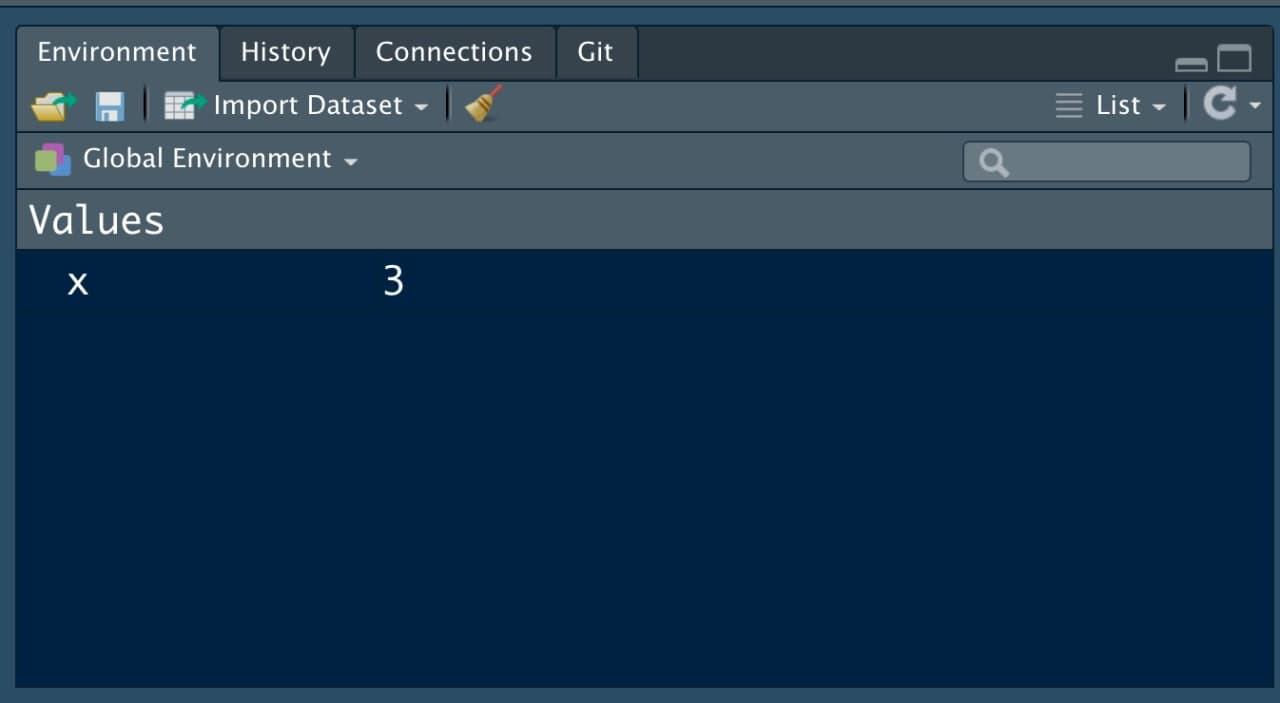
\includegraphics[width=0.75\linewidth]{./img/environment_1} 

}

\caption{Environment.}\label{fig:unnamed-chunk-8}
\end{figure}

\begin{Shaded}
\begin{Highlighting}[]
\NormalTok{y <-}\StringTok{ }\NormalTok{x }\OperatorTok{-}\StringTok{ }\DecValTok{3}
\NormalTok{x}
\end{Highlighting}
\end{Shaded}

\begin{verbatim}
## [1] 3
\end{verbatim}

\begin{Shaded}
\begin{Highlighting}[]
\NormalTok{y}
\end{Highlighting}
\end{Shaded}

\begin{verbatim}
## [1] 0
\end{verbatim}

\begin{Shaded}
\begin{Highlighting}[]
\NormalTok{x }\OperatorTok{*}\StringTok{ }\NormalTok{y}
\end{Highlighting}
\end{Shaded}

\begin{verbatim}
## [1] 0
\end{verbatim}

Dicha variable \texttt{x} además podemos reciclarla para definir, por ejemplo, una variable \texttt{y}, restándole una constante. De la misma manera que hemos hecho restas, sumas y multiplicaciones, \texttt{R} tiene todas las operaciones clásicas que podrías tener en una calculadora. Prueba a ejecutar en la consola las órdenes \texttt{x\^{}2}, \texttt{sqrt(x)} o \texttt{abs(y)}: \texttt{R} calculará las operaciones \emph{elevar al cuadrado}, \emph{raíz cuadrada} y \emph{valor absoluto} (respectivaemnte) de la variable que tengan entre paréntesis

\begin{Shaded}
\begin{Highlighting}[]
\NormalTok{x}\OperatorTok{^}\DecValTok{2}
\end{Highlighting}
\end{Shaded}

\begin{verbatim}
## [1] 9
\end{verbatim}

\begin{Shaded}
\begin{Highlighting}[]
\KeywordTok{sqrt}\NormalTok{(x)}
\end{Highlighting}
\end{Shaded}

\begin{verbatim}
## [1] 1.732051
\end{verbatim}

\begin{Shaded}
\begin{Highlighting}[]
\NormalTok{y <-}\StringTok{ }\NormalTok{x }\OperatorTok{-}\StringTok{ }\DecValTok{5}
\KeywordTok{abs}\NormalTok{(y)}
\end{Highlighting}
\end{Shaded}

\begin{verbatim}
## [1] 2
\end{verbatim}

~

\hypertarget{y-duxf3nde-programamos}{%
\section{¿Y dónde programamos?}\label{y-duxf3nde-programamos}}

\textbf{¿Estás emocionado/a? Vamos a abrir nuestro primer script}. Un \textbf{script} será el documento en el que programamos, nuestro \texttt{.doc}, pero aquí será un archivo con extensión \texttt{.R}, donde escribiremos las órdenes, que nos evitará estar lanzando todo a consola. \textbf{¿Por qué no abusar de la consola?} Una máxima para no olvidar: TODO lo que no escribas en un script, cuando cierres \texttt{RStudio}, lo habrás perdido (cómo si en lugar de escribir en un \texttt{Word} y guardarlo, nunca guardases el documento).

Para abrir nuestro primero script, haz click en el menú superior en \texttt{File\ \textless{}\textless{}\ New\ File\ \textless{}\textless{}\ R\ Script} como se muestra en la imagen \ref{fig:inicio-rstudio-5}

\begin{figure}

{\centering 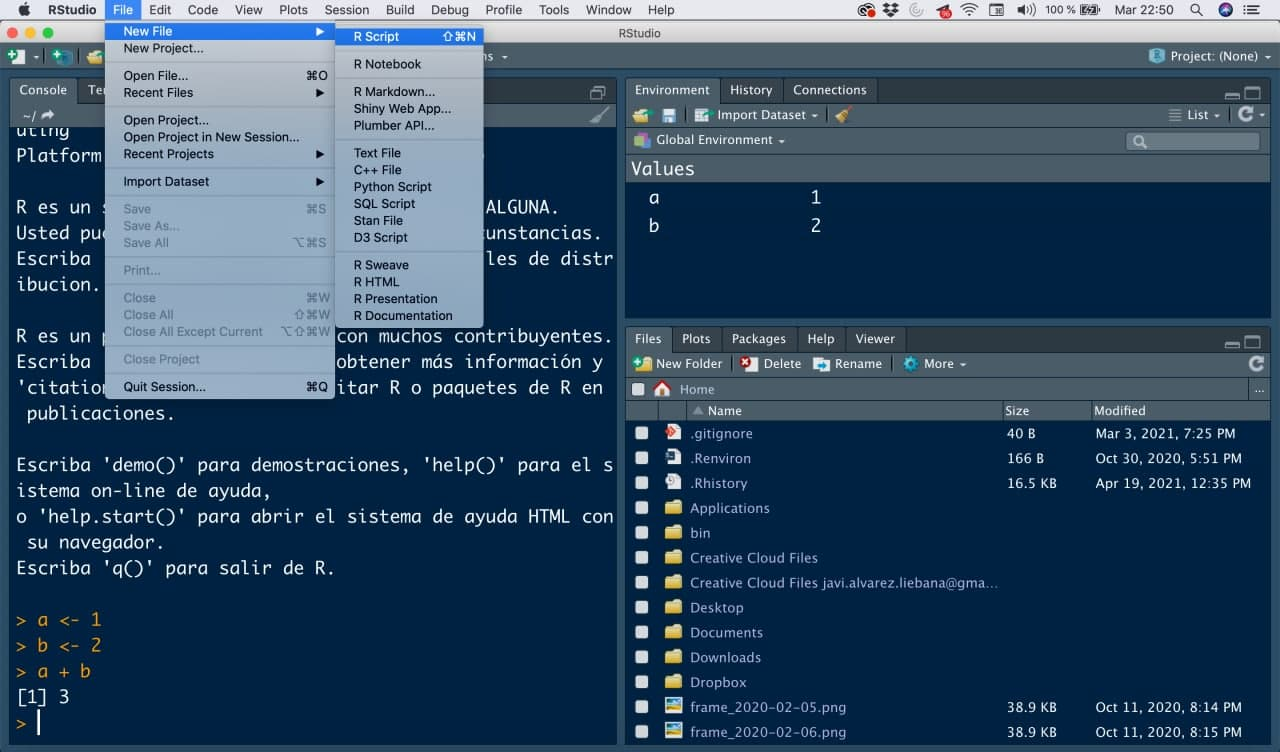
\includegraphics[width=0.8\linewidth]{./img/inicio_rstudio_5} 

}

\caption{Abriendo nuestro primer script de R.}\label{fig:inicio-rstudio-5}
\end{figure}

Tras abrirlo tendremos una cuarta ventana: esta será la ventana de nuestros códigos, la ventana más importante ya que es donde \textbf{escribiremos lo que queremos ejecutar}. Escribe el \textbf{código de la suma de arriba} en ese script y guarda el archivo haciendo click en el botón \texttt{Save\ current\ document}

\begin{Shaded}
\begin{Highlighting}[]
\NormalTok{a <-}\StringTok{ }\DecValTok{1}
\NormalTok{b <-}\DecValTok{2}
\NormalTok{a }\OperatorTok{+}\StringTok{ }\NormalTok{b}
\end{Highlighting}
\end{Shaded}

\begin{verbatim}
## [1] 3
\end{verbatim}

\begin{figure}

{\centering 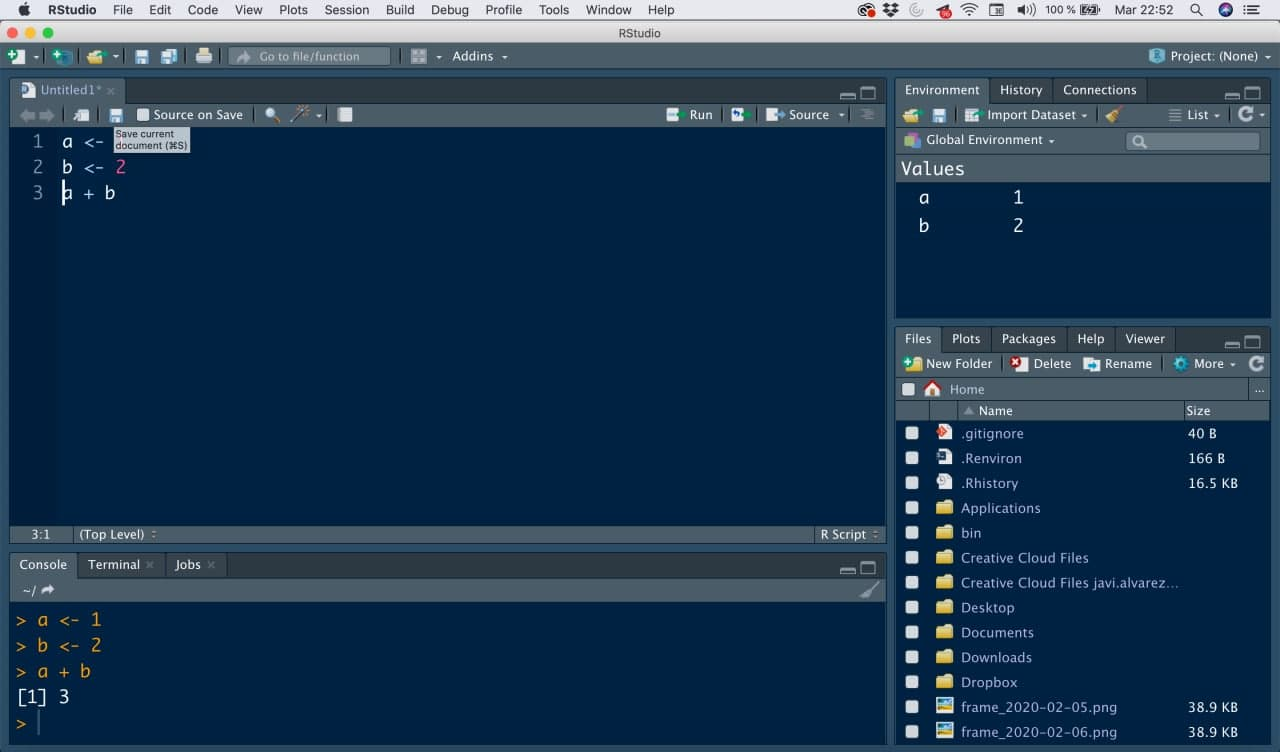
\includegraphics[width=0.85\linewidth]{./img/inicio_rstudio_6} 

}

\caption{Escribiendo y guardando nuestro primer script.}\label{fig:inicio-rstudio-6}
\end{figure}

Ese código no se ejecuta salvo que se lo digamos. Tenemos \textbf{tres opciones para ejecutar código}:

\begin{itemize}
\item
  \textbf{\textcolor{#20935E}{Copiar y pegar el trozo de código en la consola}} (como hemos hecho al principio).
\item
  \textbf{\textcolor{#20935E}{Seleccionar líneas de código y clickar en Run}} (o con su atajo de teclado), lo que hará que se ejecute solo las líneas seleccionadas.
\item
  \textbf{\textcolor{#20935E}{Activar el cuadrado Source on save a la derecha del botón de guardar}} y volvemos a hacer click en el botón de guardar: siempre que esa opción esté activada, al guardar no solo es nos guarda el archivo \texttt{.R} sino que además \textbf{se ejecuta} el código completo que tengas en el script.
\end{itemize}

\hypertarget{tipos_errores}{%
\section{Tipos de errores}\label{tipos_errores}}

Durante tu aprendizaje en \texttt{R} va a ser \textbf{muy habitual} que las cosas no salgan a la primera, \textbf{apareciendo en consola mensajes en un color rojo}. Un \textbf{miedo} muy habitual cuando se empieza a programar es pensar que si haces algo mal o aparece algún mensaje de error, el ordenador puede explotar en cualquier momento. \textbf{A programar se aprende programando}, así que haz las pruebas que quieras, lo peor que puede pasar es que necesites cerrar sesión en \texttt{R\ Studio} y abrirlo de nuevo, o en el peor de los casos, desintalarlo y volverlo a iinstalar.

Dado que el \(99.9\%\) de las veces tu código tendrá errores que deberás ir solventando, no está de más conocer los tipos de mensajes que \texttt{R} puede sacarte por consola.

Los \textbf{\textcolor{#dc3545}{mensajes de ERROR}} irán precedidos de la frase \textbf{\textcolor{#dc3545}{«Error in...»}}, dándote a veces incluso el tipo de error y la línea de código en la que se ha producido. Veamos un ejemplo intentando sumar un número a una cadena de texto.

\begin{Shaded}
\begin{Highlighting}[]
\StringTok{"a"} \OperatorTok{+}\StringTok{ }\DecValTok{1}
\end{Highlighting}
\end{Shaded}

\begin{verbatim}
## Error in "a" + 1: argumento no-numérico para operador binario
\end{verbatim}

Los \textbf{errores son aquellos fallos que seguramente impidan la ejecución} del código. Un \textbf{error muy habitual} es intentar acceder a alguna función de algún paquete que, o bien no tenemos instalado, o bien no hemos llamado haciendo uso del \texttt{library()}: estás intentando leerte un libro de tu biblioteca pero ni siquiera has ido a la tienda a «comprarlo».

~

Los \textbf{\textcolor{#ffc107}{mensajes de WARNING}} irán precedidos de la frase \textbf{\textcolor{#ffc107}{«Warning in...»}}, y son los fallos más delicados ya que son \textbf{posibles errores o incoherencias} que \texttt{R} detecta en tu código pero que \textbf{no van a hacer que tu código deje de ejecutarse}, aunque probablemente no lo haga como a ti te gustaría. Un ejemplo es cuando tratamos de hacer la raiz cuadrada de un número negativo.

\begin{Shaded}
\begin{Highlighting}[]
\KeywordTok{sqrt}\NormalTok{(}\OperatorTok{-}\DecValTok{1}\NormalTok{)}
\end{Highlighting}
\end{Shaded}

\begin{verbatim}
## Warning in sqrt(-1): Se han producido NaNs
\end{verbatim}

\begin{verbatim}
## [1] NaN
\end{verbatim}

¿Ha ejecutado la orden? Sí, pero te \textbf{advierte de que el resultado de la operación es un \texttt{NaN}}, un valor que no existe (al menos dentro de los números reales), un \emph{Not A Number} (ver Sección \ref{ausentes}).

~

Los \textbf{\textcolor{#20935E}{mensajes de CONTROL}} serán aquellos que aparecerán por consola sin empezar por «Error in\ldots{}» ni «Warning:\ldots{}». Dichos mensajes, que puedes incluir tú mismo en tu código con funciones como \texttt{cat()} para monitorizar la ejecución de códigos largos, no son errores ni problemas, son simplemente información que \texttt{R} considera útil aportarte.

~

\hypertarget{glosario-2}{%
\section{Glosario}\label{glosario-2}}

\textbf{\textcolor{#4197D2}{GLOSARIO}}

\begin{itemize}
\tightlist
\item
  \textbf{\textcolor{#4197D2}{Paquete}}: trozos de código realizadas por otros usuarios de la comunidad (y validades por el equipo de CRAN si la descarga es mediante \texttt{install.packages()}) para ser usados. Una vez instalados (descargados) los trozos de código a nuestro ordenador, basta con «acudir» a ellos con \texttt{library()}.
\end{itemize}

Haciendo una metáfora con la colección de libros que tengas en casa: con la \textbf{instalación hemos comprado el libro} y lo tenemos en nuestra estantería (para siempre), con la llamada al paquete, por ejemplo \texttt{library(ggplot2)}, lo que hacemos es decidir, de entre todos los libros de la estantería, cuales queremos llevarnos de viaje (en cada maleta que hagamos).

Los \textbf{paquetes usados} los verás denotados como \texttt{\{nombre\_paquete\}} a lo largo del manual.

\hypertarget{consejos-1}{%
\section{Consejos}\label{consejos-1}}

\textbf{\textcolor{#20935E}{CONSEJOS}}

~

\textbf{\textcolor{#20935E}{Panel de ayuda}}

Si escribes en la consola \texttt{?\ nombre\_funcion} (por ejemplo, escribe en la consola \texttt{?\ sqrt}), en el panel inferior derecho te aparecerá una \textbf{documentación de ayuda} de la función para saber que argumentos necesita, como puedes usar la función, qué es lo que te devuelve, ejemplos de uso, etc.

\begin{Shaded}
\begin{Highlighting}[]
\NormalTok{? sqrt}
\end{Highlighting}
\end{Shaded}

\begin{figure}

{\centering 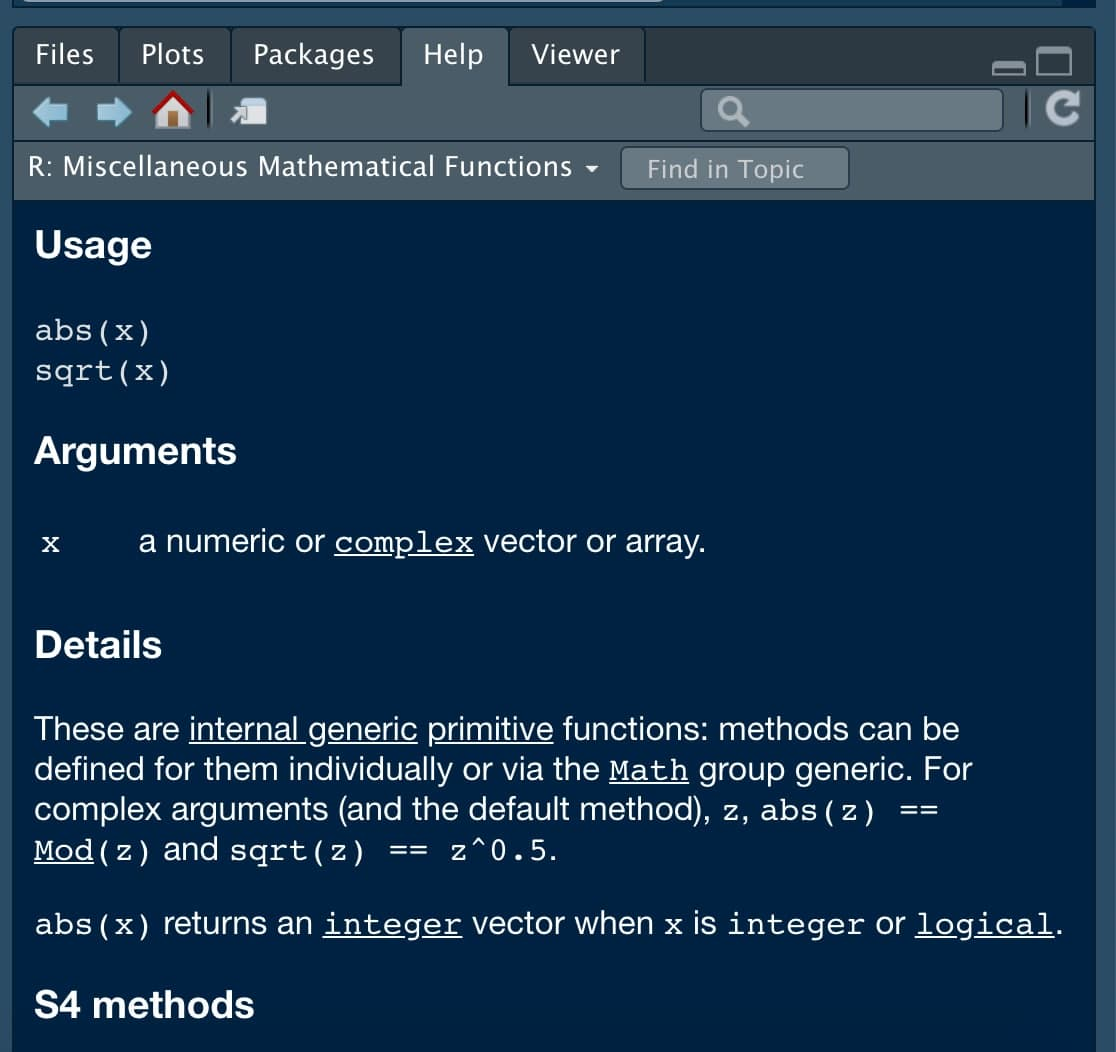
\includegraphics[width=0.5\linewidth]{./img/panel_ayuda} 

}

\caption{Panel de ayuda.}\label{fig:unnamed-chunk-15}
\end{figure}

~

\textbf{\textcolor{#20935E}{¿Cómo comentar el código?}}

Probablemente lo más importante al programar es que \textbf{te acostumbres a comentar} lo máximo posible tu código. \textbf{¿Qué es un comentario?} Es un texto que escribes entre el código precedido de \texttt{\#}: todo lo que venga detrás no será interpretado por \texttt{R} como código. Es \textbf{vital cuando programamos} que nos acostumbremos a comentar lo que hacemos, tanto para nosotros como para otras personas que puedan leer nuestro código.

~

\textbf{\textcolor{#20935E}{Índice en el código}}

Puedes escribir comentarios en el código para que automáticamente se \textbf{organice tu código en epígrafes}, mostrándote un índice en el panel lateral (haz click en el icono de la esquina superior derecha del editor) y permitiendo minimizar partes del código. Para ello puedes comentar por ejemplo con \texttt{\#\ -\/-\/-\/-\/-\ título\ -\/-\/-\/-\/-}.

\begin{figure}

{\centering 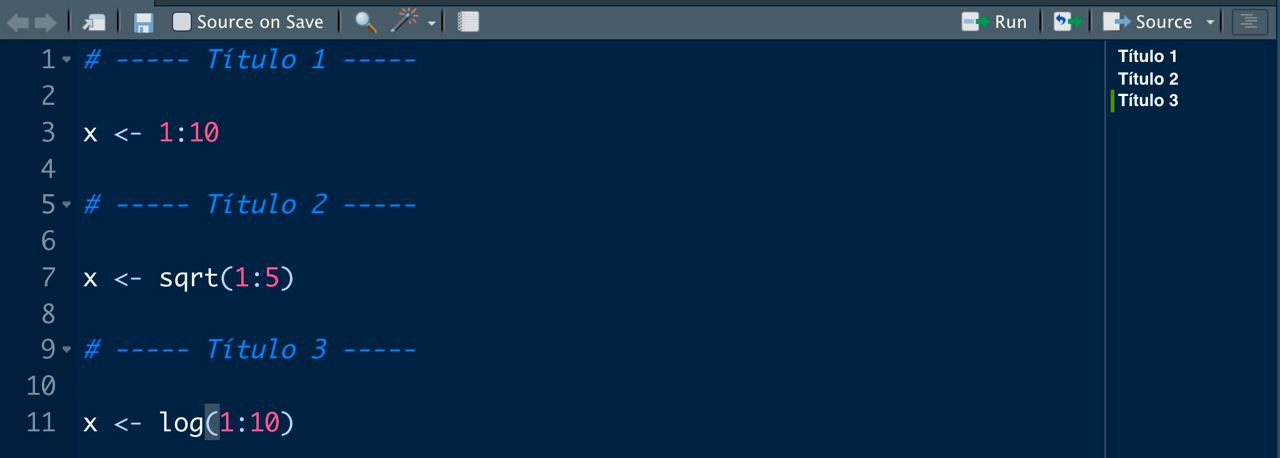
\includegraphics[width=0.7\linewidth]{./img/comentarios-indice} 

}

\caption{Comentando el código para generar un índice.}\label{fig:unnamed-chunk-16}
\end{figure}

~

\hypertarget{ejercicios}{%
\section{📝 Ejercicios}\label{ejercicios}}

(haz click en las flechas para ver soluciones)

📝Ejercicio 1: en tu consola (parte inferior de tu pantalla), asigna los valores \texttt{2} y \texttt{5} a dos variables \texttt{a} y \texttt{b}. Tras asignarles valores, multiplica los números en consola (\textbf{haz click} en la flecha para la solución propuesta).

\begin{itemize}
\tightlist
\item
  Solución:
\end{itemize}

\begin{Shaded}
\begin{Highlighting}[]
\CommentTok{# Para poner comentarios en el código se usa #}

\CommentTok{# Definición de variables}
\NormalTok{a <-}\StringTok{ }\DecValTok{2}
\NormalTok{b <-}\StringTok{ }\DecValTok{5}

\CommentTok{# Multiplicación}
\NormalTok{a }\OperatorTok{*}\StringTok{ }\NormalTok{b}
\end{Highlighting}
\end{Shaded}

\begin{verbatim}
## [1] 10
\end{verbatim}

\begin{figure}

{\centering 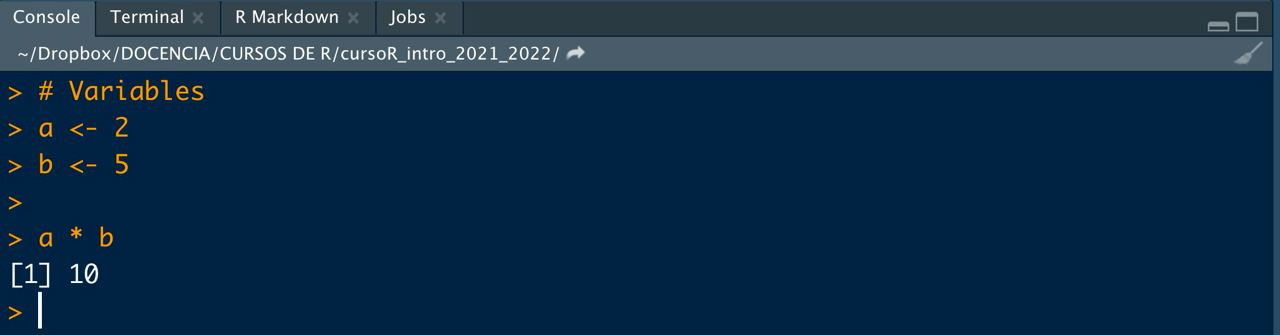
\includegraphics[width=0.8\linewidth]{./img/consola_multiplicacion} 

}

\caption{Multiplicación de a y b.}\label{fig:consola-multi}
\end{figure}

~

📝Ejercicio 2: repite el ejercicio anterior pero ahora guarda el resultado de la multiplicación en una variable \texttt{c}. Para ver el resultado guardado en \texttt{c} escribe dicha variable en consola (\textbf{haz click} en la flecha para la solución propuesta).

\begin{itemize}
\tightlist
\item
  Solución:
\end{itemize}

\begin{Shaded}
\begin{Highlighting}[]
\CommentTok{# Variables}
\NormalTok{a <-}\StringTok{ }\DecValTok{2}
\NormalTok{b <-}\StringTok{ }\DecValTok{5}

\CommentTok{# Resultado}
\NormalTok{c <-}\StringTok{ }\NormalTok{a }\OperatorTok{*}\StringTok{ }\NormalTok{b}

\CommentTok{# Muestro en consola}
\NormalTok{c}
\end{Highlighting}
\end{Shaded}

\begin{verbatim}
## [1] 10
\end{verbatim}

\begin{figure}

{\centering 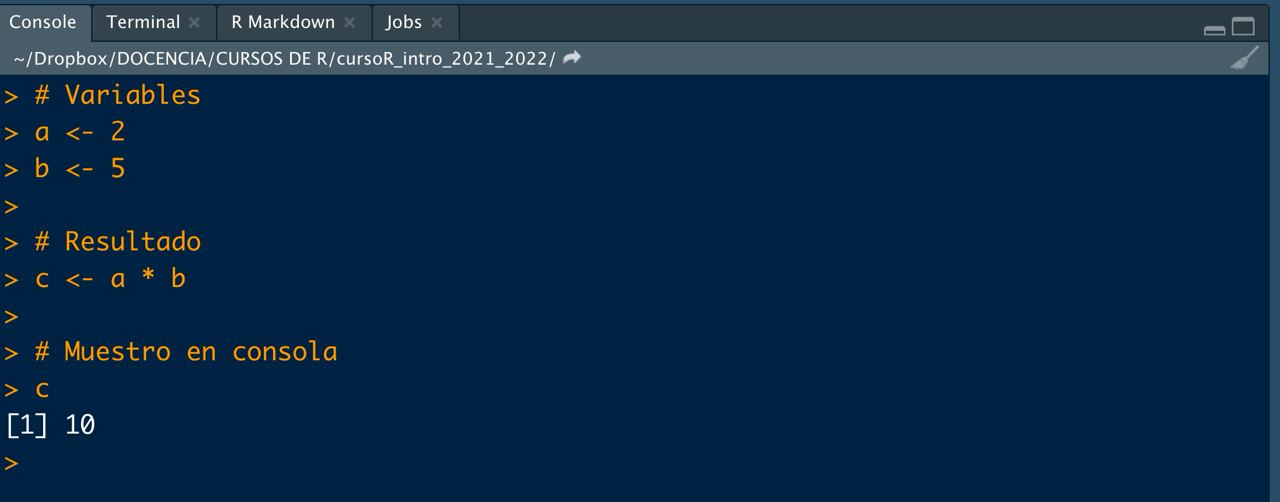
\includegraphics[width=0.8\linewidth]{./img/consola_multiplicacion_2} 

}

\caption{Multiplicación de a y b guardando el resultado.}\label{fig:consola-multi-2}
\end{figure}

~

📝Ejercicio 3: asigna ahora los valores \texttt{1}, \texttt{-2}, \texttt{3} a tres variables \texttt{a}, \texttt{b} y \texttt{c}, y calcula la raíz cuadrada de cada uno.

\begin{itemize}
\tightlist
\item
  Solución:
\end{itemize}

\begin{Shaded}
\begin{Highlighting}[]
\CommentTok{# Variables}
\NormalTok{a <-}\StringTok{ }\DecValTok{1}
\NormalTok{b <-}\StringTok{ }\DecValTok{-2}
\NormalTok{c <-}\StringTok{ }\DecValTok{3}

\CommentTok{# Resultado}
\KeywordTok{sqrt}\NormalTok{(a)}
\end{Highlighting}
\end{Shaded}

\begin{verbatim}
## [1] 1
\end{verbatim}

\begin{Shaded}
\begin{Highlighting}[]
\KeywordTok{sqrt}\NormalTok{(b)}
\end{Highlighting}
\end{Shaded}

\begin{verbatim}
## [1] NaN
\end{verbatim}

\begin{Shaded}
\begin{Highlighting}[]
\KeywordTok{sqrt}\NormalTok{(c)}
\end{Highlighting}
\end{Shaded}

\begin{verbatim}
## [1] 1.732051
\end{verbatim}

~

📝Ejercicio 4: repite el ejercicio 2 pero ahora escribe el código en un script (fichero \texttt{.R}, guardado en \href{https://github.com/dadosdelaplace/courses-ECI-2022/blob/main/scripts/script01.R}{\textbf{script01.R}}). Recuerda al acabar seleccionar las líneas a ejecutar y clickar \texttt{Run}, o bien guardar el script con \texttt{Source\ on\ save} activado (\textbf{haz click} en la flecha para la solución propuesta).

\begin{itemize}
\tightlist
\item
  Solución:
\end{itemize}

\begin{figure}

{\centering 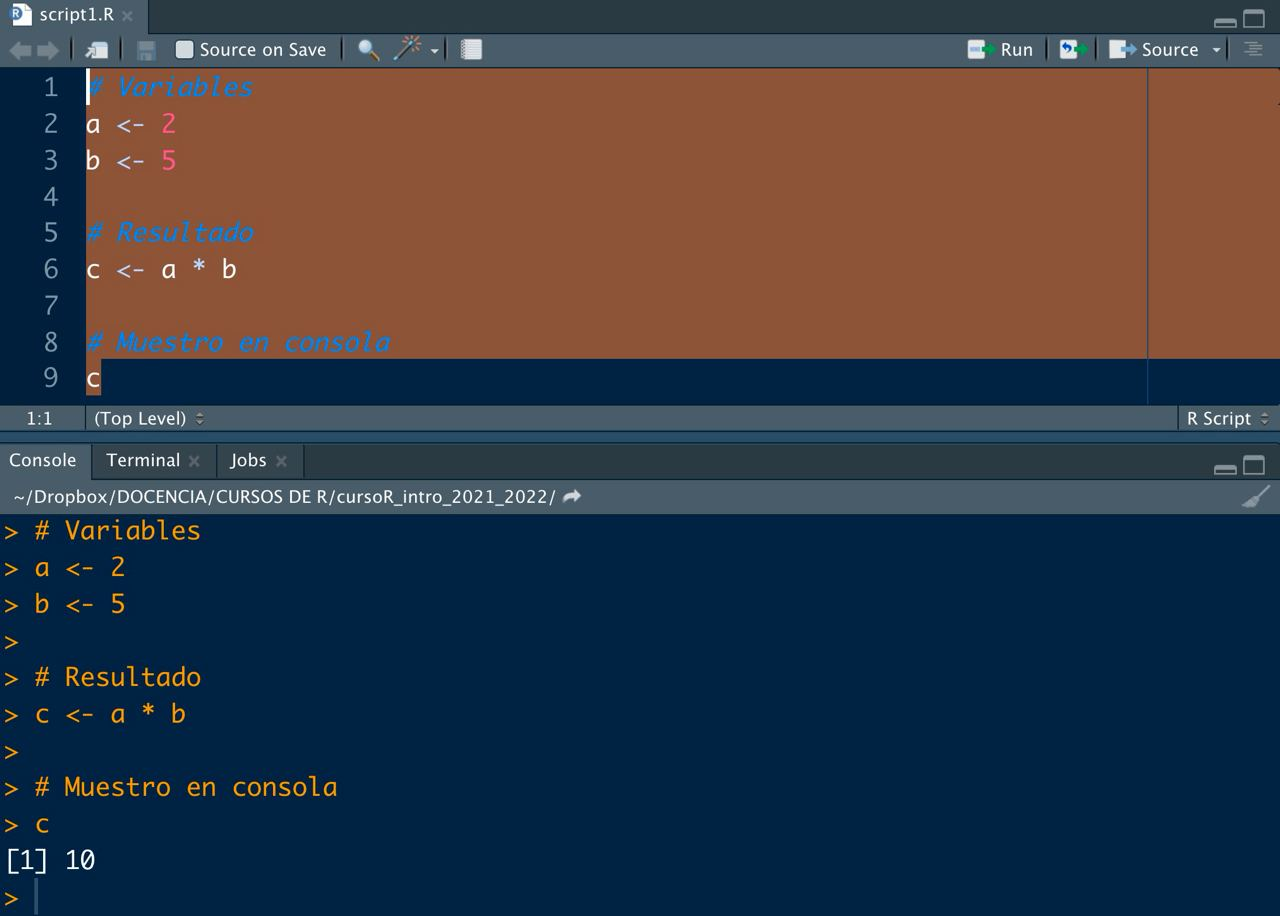
\includegraphics[width=0.8\linewidth]{./img/consola_multiplicacion_3} 

}

\caption{Multiplicación de a y b guardando el resultado pero escribiendo en el script.}\label{fig:consola-multi-3}
\end{figure}

~

📝Ejercicio 5: calcula en consola la suma de 3 más 4, y todo ello multiplicado por 10, y asígnalo a una variable \texttt{x} (\textbf{haz click} en la flecha para la solución propuesta).

\begin{itemize}
\tightlist
\item
  Solución:
\end{itemize}

\begin{Shaded}
\begin{Highlighting}[]
\NormalTok{x <-}\StringTok{ }\NormalTok{(}\DecValTok{3} \OperatorTok{+}\StringTok{ }\DecValTok{4}\NormalTok{) }\OperatorTok{*}\StringTok{ }\DecValTok{10}
\end{Highlighting}
\end{Shaded}

~

📝Ejercicio 6: asigna un valor positivo a \texttt{x} y calcula su raíz cuadrada; asigna otro negativo y calcula su valor absoluto (\textbf{haz click} en la flecha para la solución propuesta).

\begin{itemize}
\tightlist
\item
  Solución:
\end{itemize}

\begin{Shaded}
\begin{Highlighting}[]
\CommentTok{# Raíz cuadrada}
\NormalTok{x <-}\StringTok{ }\DecValTok{73}
\KeywordTok{sqrt}\NormalTok{(x)}
\end{Highlighting}
\end{Shaded}

\begin{verbatim}
## [1] 8.544004
\end{verbatim}

\begin{Shaded}
\begin{Highlighting}[]
\CommentTok{# Valor absoluto}
\NormalTok{y <-}\StringTok{ }\DecValTok{-73}
\KeywordTok{abs}\NormalTok{(y)}
\end{Highlighting}
\end{Shaded}

\begin{verbatim}
## [1] 73
\end{verbatim}

~

\textbf{\textcolor{#20935E}{CONSEJO:}}

Las órdenes \texttt{sqrt(x)} y \texttt{abs(y)} se llaman \textbf{funciones}, y la variable que tienen entre paréntesis se llama \textbf{argumento de la función}: una variable que toma de entrada la función y con la que opera internamente.

~

📝Ejercicio 7: usando la variable \texttt{x} ya definida, calcula \texttt{x\ -\ 5} y guárdalo en una nueva variable \texttt{z} (\textbf{haz click} en la flecha para la solución propuesta).

\begin{itemize}
\tightlist
\item
  Solución:
\end{itemize}

\begin{Shaded}
\begin{Highlighting}[]
\NormalTok{z <-}\StringTok{ }\NormalTok{x }\OperatorTok{-}\StringTok{ }\DecValTok{5}
\NormalTok{z}
\end{Highlighting}
\end{Shaded}

\begin{verbatim}
## [1] 68
\end{verbatim}

~

📝Ejercicio 8: usando las variables \texttt{x} y \texttt{z} ya definidas, calcula la raíz cuadrada del máximo entre ambas, y guárdalo en una nueva variable \texttt{t}. Hazlo en un script en lugar de en consola (\textbf{haz click} en la flecha para la solución propuesta).

\begin{itemize}
\tightlist
\item
  Solución:
\end{itemize}

\begin{Shaded}
\begin{Highlighting}[]
\NormalTok{t <-}\StringTok{ }\KeywordTok{sqrt}\NormalTok{(}\KeywordTok{max}\NormalTok{(x, z)) }
\NormalTok{t}
\end{Highlighting}
\end{Shaded}

\begin{verbatim}
## [1] 8.544004
\end{verbatim}

~

\textbf{\textcolor{#ffc107}{WARNING:}}

No hace falta gastar una línea por cada orden que quieras ejecutar. Tampoco necesitas guardar cada paso intermedio que realices. \textbf{\textcolor{#ffc107}{Cuidado con la memoria}}: cada asignación que hagas es una variable guardada que consume recursos en tu ordenador.

\hypertarget{part-conceptos-buxe1sicos}{%
\part{Conceptos básicos}\label{part-conceptos-buxe1sicos}}

\hypertarget{tipos-datos}{%
\chapter{Tipos de datos}\label{tipos-datos}}

\begin{blackbox}

Scripts usados:

\begin{itemize}
\tightlist
\item
  \href{https://github.com/dadosdelaplace/courses-ECI-2022/blob/main/scripts/script02.R}{\textbf{script02.R}}: tipos de datos y funciones usadas con ellos. Ver en \url{https://github.com/dadosdelaplace/courses-ECI-2022/blob/main/scripts/script02.R}
\end{itemize}


\end{blackbox}

~

Tras las lecciones anteriores, los ejercicios planteados y lo que hayas jugueteado por tu cuenta, deberíamos saber usar ya \texttt{R} como una calculadora. Vamos a ir más allá: \textbf{¿existen datos más allá de los números?} En este capítulo vamos a empezar a familiarizarnos con los tipos de datos (individuales) que podemos necesitar. Piensa por ejemplo en los datos guardados de una persona:

\begin{itemize}
\tightlist
\item
  La edad será un \textbf{número (sin decimales)}
\item
  Su peso o estatura será otro \textbf{número (ahora con decimales)}.
\item
  Su nombre será una \textbf{cadena de texto}.
\item
  Su fecha de nacimiento será precisamente eso, una \textbf{fecha}.
\item
  A la pregunta «¿está usted soltero/a?» la respuesta será lo que llamamos una \textbf{variable binaria}: una variable que solo puede valer \texttt{TRUE} (si está soltero/a) y \texttt{FALSE} (en otro caso).
\end{itemize}

Existen \textbf{más tipos} (como números complejos) pero con estos nos valdrá para nuestra introducción.

\hypertarget{numericas}{%
\section{Variables numéricas}\label{numericas}}

\begin{itemize}
\tightlist
\item
  {[}X{]} Variables numéricas (individuales)
\item
  {[} {]} Variables de caracteres
\item
  {[} {]} Variables lógicas
\item
  {[} {]} Variables de tipo fecha
\end{itemize}

Probablemente el dato \textbf{más sencillo y obvio} de entender sean los datos numéricos, datos que ya hemos usado en nuestros primeros pasos como calculadora.

\begin{Shaded}
\begin{Highlighting}[]
\NormalTok{a <-}\StringTok{ }\DecValTok{1}
\NormalTok{b <-}\StringTok{ }\DecValTok{2}
\NormalTok{a }\OperatorTok{+}\StringTok{ }\NormalTok{b}
\end{Highlighting}
\end{Shaded}

\begin{verbatim}
## [1] 3
\end{verbatim}

En el código anterior, tanto \texttt{a} como \texttt{b} como la suma \texttt{a\ +\ b} son de \textbf{tipo numérico}, algo que podemos comprobar con la función \texttt{class()} (nos devuelve \emph{numeric}).

\begin{Shaded}
\begin{Highlighting}[]
\CommentTok{# Clase de las variables}
\KeywordTok{class}\NormalTok{(a)}
\end{Highlighting}
\end{Shaded}

\begin{verbatim}
## [1] "numeric"
\end{verbatim}

\begin{Shaded}
\begin{Highlighting}[]
\KeywordTok{class}\NormalTok{(b)}
\end{Highlighting}
\end{Shaded}

\begin{verbatim}
## [1] "numeric"
\end{verbatim}

\begin{Shaded}
\begin{Highlighting}[]
\KeywordTok{class}\NormalTok{(a }\OperatorTok{+}\StringTok{ }\NormalTok{b)}
\end{Highlighting}
\end{Shaded}

\begin{verbatim}
## [1] "numeric"
\end{verbatim}

También podemos comprobar su naturaleza con \texttt{typeof()}, que nos devuelve la naturaleza del dato tal cual es guardada en \texttt{R}.

\begin{Shaded}
\begin{Highlighting}[]
\CommentTok{# Topología interna}
\KeywordTok{typeof}\NormalTok{(a)}
\end{Highlighting}
\end{Shaded}

\begin{verbatim}
## [1] "double"
\end{verbatim}

\begin{Shaded}
\begin{Highlighting}[]
\KeywordTok{typeof}\NormalTok{(b)}
\end{Highlighting}
\end{Shaded}

\begin{verbatim}
## [1] "double"
\end{verbatim}

\begin{Shaded}
\begin{Highlighting}[]
\KeywordTok{typeof}\NormalTok{(a }\OperatorTok{+}\StringTok{ }\NormalTok{b)}
\end{Highlighting}
\end{Shaded}

\begin{verbatim}
## [1] "double"
\end{verbatim}

Fíjate que ambas órdenes combinadas nos dicen que las variables son de tipo numérico pero concretamente de tipo \emph{double}: dichas variables son entendidas internamente como números con decimales (aunque no los veamos), lo que en \textbf{matemáticas se llaman números reales} (por curiosidad: el término \emph{double} viene de lenguajes de programación antiguos como \texttt{C}, que significa «doble precisión», para indicarle que reserve 8 bytes - 64 bits - de memoria). Durante el curso no distinguiremos entre distintos tipos de números, para nosotros serán siempre de clase \emph{numeric} y de tipo \emph{double}, pero podríamos definir números enteros o \emph{integer} (sin decimales, ahorrando huecos en memoria).

\begin{Shaded}
\begin{Highlighting}[]
\CommentTok{# Dato numérico (entero)}
\NormalTok{a <-}\StringTok{ }\NormalTok{1L}
\KeywordTok{class}\NormalTok{(a)}
\end{Highlighting}
\end{Shaded}

\begin{verbatim}
## [1] "integer"
\end{verbatim}

\begin{Shaded}
\begin{Highlighting}[]
\KeywordTok{typeof}\NormalTok{(a)}
\end{Highlighting}
\end{Shaded}

\begin{verbatim}
## [1] "integer"
\end{verbatim}

Con los \textbf{datos numéricos} podemos realizar todas las \textbf{operaciones} que se nos ocurriría hacer en una \textbf{calculadora}, como sumar (\texttt{+}), restar (\texttt{-}), multiplicar (\texttt{*}), dividir (\texttt{/}), raíz cuadrada (\texttt{sqrt()}), valor absoluto (\texttt{abs()}), elevar al cuadrado (\texttt{\^{}2}), elevar al cubo (\texttt{\^{}3}), etc.

\begin{Shaded}
\begin{Highlighting}[]
\CommentTok{# Definimos dos variables numéricas}
\NormalTok{a <-}\StringTok{ }\DecValTok{1}
\NormalTok{b <-}\StringTok{ }\DecValTok{-2}

\CommentTok{# Suma y resta}
\NormalTok{a }\OperatorTok{+}\StringTok{ }\NormalTok{b}
\end{Highlighting}
\end{Shaded}

\begin{verbatim}
## [1] -1
\end{verbatim}

\begin{Shaded}
\begin{Highlighting}[]
\NormalTok{a }\OperatorTok{-}\StringTok{ }\NormalTok{b}
\end{Highlighting}
\end{Shaded}

\begin{verbatim}
## [1] 3
\end{verbatim}

\begin{Shaded}
\begin{Highlighting}[]
\CommentTok{# Multiplicación y división}
\NormalTok{a }\OperatorTok{*}\StringTok{ }\NormalTok{b}
\end{Highlighting}
\end{Shaded}

\begin{verbatim}
## [1] -2
\end{verbatim}

\begin{Shaded}
\begin{Highlighting}[]
\NormalTok{a }\OperatorTok{/}\StringTok{ }\NormalTok{b}
\end{Highlighting}
\end{Shaded}

\begin{verbatim}
## [1] -0.5
\end{verbatim}

\begin{Shaded}
\begin{Highlighting}[]
\CommentTok{# Raíz cuadrada}
\KeywordTok{sqrt}\NormalTok{(a)}
\end{Highlighting}
\end{Shaded}

\begin{verbatim}
## [1] 1
\end{verbatim}

\begin{Shaded}
\begin{Highlighting}[]
\CommentTok{# Valor absoluto}
\KeywordTok{abs}\NormalTok{(b)}
\end{Highlighting}
\end{Shaded}

\begin{verbatim}
## [1] 2
\end{verbatim}

\begin{Shaded}
\begin{Highlighting}[]
\CommentTok{# Potencias}
\NormalTok{a}\OperatorTok{^}\DecValTok{2}
\end{Highlighting}
\end{Shaded}

\begin{verbatim}
## [1] 1
\end{verbatim}

\begin{Shaded}
\begin{Highlighting}[]
\NormalTok{b}\OperatorTok{^}\DecValTok{3}
\end{Highlighting}
\end{Shaded}

\begin{verbatim}
## [1] -8
\end{verbatim}

\hypertarget{caracter}{%
\section{Variables de tipo caracter (texto)}\label{caracter}}

\begin{itemize}
\tightlist
\item
  {[}X{]} Variables numéricas (individuales)
\item
  {[}X{]} Variables de caracteres
\item
  {[} {]} Variables lógicas
\item
  {[} {]} Variables de tipo fecha
\end{itemize}

Pero no solo de números viven los datos: imagina que además de la edad de una persona queremos guardar su nombre.

\begin{Shaded}
\begin{Highlighting}[]
\NormalTok{edad <-}\StringTok{ }\DecValTok{32}
\NormalTok{nombre <-}\StringTok{ "Javier"}

\KeywordTok{class}\NormalTok{(edad)}
\end{Highlighting}
\end{Shaded}

\begin{verbatim}
## [1] "numeric"
\end{verbatim}

\begin{Shaded}
\begin{Highlighting}[]
\KeywordTok{typeof}\NormalTok{(edad)}
\end{Highlighting}
\end{Shaded}

\begin{verbatim}
## [1] "double"
\end{verbatim}

\begin{Shaded}
\begin{Highlighting}[]
\KeywordTok{class}\NormalTok{(nombre)}
\end{Highlighting}
\end{Shaded}

\begin{verbatim}
## [1] "character"
\end{verbatim}

\begin{Shaded}
\begin{Highlighting}[]
\KeywordTok{typeof}\NormalTok{(nombre)}
\end{Highlighting}
\end{Shaded}

\begin{verbatim}
## [1] "character"
\end{verbatim}

Fíjate que ahora tenemos en \texttt{nombre} una variable de tipo \emph{character}, es decir, una cadena de texto (conocido en otros lenguajes como \emph{string} o \emph{char}): \textbf{letras y caracteres entre comillas}.

\hypertarget{nuestra-primera-funciuxf3n-pastepaste0}{%
\subsection{Nuestra primera función: paste/paste0}\label{nuestra-primera-funciuxf3n-pastepaste0}}

Las \textbf{cadenas de texto} son un tipo especial de dato, con los que obviamente no podremos hacer operaciones aritméticas, pero si podemos hacer operaciones propias de cadenas de texto como puede ser la función \texttt{paste()}. Dicha función nos permite \textbf{pegar dos cadenas de caracteres}, decidiendo que caracter queremos que vaya entre palabra con el argumento \texttt{sep\ =}.

\begin{Shaded}
\begin{Highlighting}[]
\NormalTok{nombre <-}\StringTok{ "Javier"}
\NormalTok{apellido <-}\StringTok{ "Álvarez"}
\KeywordTok{paste}\NormalTok{(nombre, apellido, }\DataTypeTok{sep =} \StringTok{""}\NormalTok{) }\CommentTok{# todo junto}
\end{Highlighting}
\end{Shaded}

\begin{verbatim}
## [1] "JavierÁlvarez"
\end{verbatim}

\begin{Shaded}
\begin{Highlighting}[]
\KeywordTok{paste}\NormalTok{(nombre, apellido, }\DataTypeTok{sep =} \StringTok{" "}\NormalTok{) }\CommentTok{# separados por un espacio}
\end{Highlighting}
\end{Shaded}

\begin{verbatim}
## [1] "Javier Álvarez"
\end{verbatim}

\begin{Shaded}
\begin{Highlighting}[]
\KeywordTok{paste}\NormalTok{(nombre, apellido, }\DataTypeTok{sep =} \StringTok{"."}\NormalTok{) }\CommentTok{# separados por un punto .}
\end{Highlighting}
\end{Shaded}

\begin{verbatim}
## [1] "Javier.Álvarez"
\end{verbatim}

Si queremos pegar cadenas de texto sin ningún tipo de caracter, existe una forma más abreviada y limpia de ejecutar la orden, usando la función \texttt{paste0()}

\begin{Shaded}
\begin{Highlighting}[]
\CommentTok{# Son equivalentes}
\KeywordTok{paste}\NormalTok{(nombre, apellido, }\DataTypeTok{sep =} \StringTok{""}\NormalTok{) }\CommentTok{# todo junto}
\end{Highlighting}
\end{Shaded}

\begin{verbatim}
## [1] "JavierÁlvarez"
\end{verbatim}

\begin{Shaded}
\begin{Highlighting}[]
\KeywordTok{paste0}\NormalTok{(nombre, apellido) }\CommentTok{# todo junto sin nada separando}
\end{Highlighting}
\end{Shaded}

\begin{verbatim}
## [1] "JavierÁlvarez"
\end{verbatim}

Cuando hemos ejecutado \texttt{paste()} estamos ejecutando lo que se conoce como una \textbf{función}: una palabra reservada que representa un \textbf{conjunto de órdenes}, y que se ejecuta a partir de unos \textbf{argumentos de entrada}. En el caso de la función \texttt{paste()} puede tener varios argumentos: las cadenas de texto que queremos copiar, y un \textbf{argumento opcional} llamado \texttt{sep}, que podemos darle un valor con concreto o dejarlo sin especificar. Lo que hará \texttt{R} será tomar su \textbf{valor por defecto} igual a \texttt{sep\ =\ "\ "} (por defecto, la función \texttt{paste()} pega cadenas de texto con un espacio entre ellas). Prueba a ejecutar \texttt{?\ paste} en consola para ver las opciones en el \textbf{panel de ayuda}.

\begin{Shaded}
\begin{Highlighting}[]
\CommentTok{# Son equivalentes}
\KeywordTok{paste}\NormalTok{(nombre, apellido, }\DataTypeTok{sep =} \StringTok{" "}\NormalTok{)}
\end{Highlighting}
\end{Shaded}

\begin{verbatim}
## [1] "Javier Álvarez"
\end{verbatim}

\begin{Shaded}
\begin{Highlighting}[]
\KeywordTok{paste}\NormalTok{(nombre, apellido)}
\end{Highlighting}
\end{Shaded}

\begin{verbatim}
## [1] "Javier Álvarez"
\end{verbatim}

\hypertarget{nuestro-primer-paquete-glue}{%
\subsection{Nuestro primer paquete: glue}\label{nuestro-primer-paquete-glue}}

Otra \textbf{forma más intuitiva de trabajar con textos y variables numéricas} es usar el paquete \texttt{\{glue\}}, que nos permite pegar cadenas de texto a variables numéricas de \textbf{forma simbólica}.

\begin{Shaded}
\begin{Highlighting}[]
\KeywordTok{install.packages}\NormalTok{(}\StringTok{"glue"}\NormalTok{) }\CommentTok{# solo la primera vez}
\end{Highlighting}
\end{Shaded}

\begin{Shaded}
\begin{Highlighting}[]
\KeywordTok{library}\NormalTok{(glue)}
\end{Highlighting}
\end{Shaded}

Recuerda que \texttt{install.packages()} es solo necesario la primera que «compramos el libro»: nos bajamos una serie de archivos a nuestro ordenador. Una vez que hemos comprado el libro, cada vez que queramos usarlo bastará con indicarle que nos traiga ese libro concreto con \texttt{library()}.

El paquete \texttt{\{glue\}} nos permite pegar de una forma mucho más legible cadenas de texto

\begin{Shaded}
\begin{Highlighting}[]
\CommentTok{# Ejemplo 1}
\NormalTok{edad <-}\StringTok{ }\DecValTok{32}
\KeywordTok{glue}\NormalTok{(}\StringTok{"La edad es de \{edad\} años"}\NormalTok{)}
\end{Highlighting}
\end{Shaded}

\begin{verbatim}
## La edad es de 32 años
\end{verbatim}

\begin{Shaded}
\begin{Highlighting}[]
\KeywordTok{paste}\NormalTok{(}\StringTok{"La edad es de"}\NormalTok{, edad, }\StringTok{"años"}\NormalTok{) }\CommentTok{# equivalente}
\end{Highlighting}
\end{Shaded}

\begin{verbatim}
## [1] "La edad es de 32 años"
\end{verbatim}

\begin{Shaded}
\begin{Highlighting}[]
\CommentTok{# Ejemplo 2}
\NormalTok{edad <-}\StringTok{ }\DecValTok{32}
\NormalTok{unidades <-}\StringTok{ "años"}
\KeywordTok{glue}\NormalTok{(}\StringTok{"La edad es de \{edad\} \{unidades\}"}\NormalTok{)}
\end{Highlighting}
\end{Shaded}

\begin{verbatim}
## La edad es de 32 años
\end{verbatim}

También podemos hacer uso de dicha función sin tener los valores numéricos previamente guardados en variables.

\begin{Shaded}
\begin{Highlighting}[]
\CommentTok{# Otra forma sin definir variables a priori}
\KeywordTok{glue}\NormalTok{(}\StringTok{"La edad es de \{32\} años"}\NormalTok{)}
\end{Highlighting}
\end{Shaded}

\begin{verbatim}
## La edad es de 32 años
\end{verbatim}

~

\hypertarget{logicas}{%
\section{Variables lógicas (TRUE/FALSE)}\label{logicas}}

\begin{itemize}
\tightlist
\item
  {[}X{]} Variables numéricas (individuales)
\item
  {[}X{]} Variables de caracteres
\item
  {[}X{]} Variables lógicas
\item
  {[} {]} Variables de tipo fecha
\end{itemize}

Probablemente el tipo de datos más importante en todo lenguaje de programación son las \textbf{variables lógicas}. Un \textbf{valor lógico} puede tomar \textbf{dos valores} (en realidad pueden tomar un tercer valor, \texttt{NA}, las siglas de \emph{not available} para representar datos ausentes, pero lo veremos más adelante):

\begin{itemize}
\tightlist
\item
  \texttt{TRUE} (guardado internamente como un \texttt{1}).
\item
  \texttt{FALSE} (guardado internamente como un \texttt{0}).
\end{itemize}

Este tipo de variables, también conocidas como \textbf{variables binarias (solo dos valores) o booleanas}, son la base de la programación ya que cada bit de nuestro ordenador puede guardar un \texttt{1} o un \texttt{0}.

\begin{Shaded}
\begin{Highlighting}[]
\NormalTok{soltero <-}\StringTok{ }\OtherTok{TRUE} \CommentTok{# ¿Es soltero? --> SÍ}
\NormalTok{carnet_conducir <-}\StringTok{ }\OtherTok{FALSE} \CommentTok{# ¿Tiene carnet de conducir? --> NO}

\KeywordTok{class}\NormalTok{(soltero)}
\end{Highlighting}
\end{Shaded}

\begin{verbatim}
## [1] "logical"
\end{verbatim}

\begin{Shaded}
\begin{Highlighting}[]
\KeywordTok{typeof}\NormalTok{(soltero)}
\end{Highlighting}
\end{Shaded}

\begin{verbatim}
## [1] "logical"
\end{verbatim}

\begin{Shaded}
\begin{Highlighting}[]
\KeywordTok{class}\NormalTok{(carnet_conducir)}
\end{Highlighting}
\end{Shaded}

\begin{verbatim}
## [1] "logical"
\end{verbatim}

\begin{Shaded}
\begin{Highlighting}[]
\KeywordTok{typeof}\NormalTok{(carnet_conducir)}
\end{Highlighting}
\end{Shaded}

\begin{verbatim}
## [1] "logical"
\end{verbatim}

Ahora nuestas variables son guardadas como \emph{logical}, y pueden tomar los valores \texttt{TRUE/FALSE}, aunque internamente son guardados como \texttt{1/0}. Es importante entender que \textbf{no son variables de texto}:

\begin{itemize}
\tightlist
\item
  \texttt{"TRUE"} es un texto (internamente idéntico a \texttt{rojo} o \texttt{azul})
\item
  \texttt{TRUE} es una variable lógica
\end{itemize}

\begin{Shaded}
\begin{Highlighting}[]
\CommentTok{# Texto}
\NormalTok{texto <-}\StringTok{ "TRUE"}
\NormalTok{texto }\OperatorTok{+}\StringTok{ }\DecValTok{1}
\end{Highlighting}
\end{Shaded}

\begin{verbatim}
## Error in texto + 1: argumento no-numérico para operador binario
\end{verbatim}

\begin{Shaded}
\begin{Highlighting}[]
\CommentTok{# Lógica}
\NormalTok{logica <-}\StringTok{ }\OtherTok{TRUE}
\NormalTok{logica }\OperatorTok{+}\StringTok{ }\DecValTok{1}
\end{Highlighting}
\end{Shaded}

\begin{verbatim}
## [1] 2
\end{verbatim}

Estos valores suelen ser resultado de evaluar \textbf{condiciones lógicas}. Por ejemplo, imaginemos que queremos comprobar si una persona está soltero o no, y si tiene carnet de conducir o no. Basta con que ejecutemos la orden \texttt{soltero\ ==\ TRUE}, que nos devolverá \texttt{TRUE} si está soltero, y \texttt{FALSE} en caso contrario. De igual manera podremos hacer \texttt{carnet\_conducir\ ==\ TRUE}. \textbf{IMPORTANTE}: cuando queremos \textbf{comparar si un elemento es igual a otro}, usaremos el operador de comparación \texttt{==}, pudiendo usar también su opuesto \texttt{!=} («distinto de»).

\begin{Shaded}
\begin{Highlighting}[]
\NormalTok{soltero }\OperatorTok{==}\StringTok{ }\OtherTok{TRUE}
\end{Highlighting}
\end{Shaded}

\begin{verbatim}
## [1] TRUE
\end{verbatim}

\begin{Shaded}
\begin{Highlighting}[]
\NormalTok{soltero }\OperatorTok{!=}\StringTok{ }\OtherTok{TRUE} \CommentTok{# igual que soltero == FALSE}
\end{Highlighting}
\end{Shaded}

\begin{verbatim}
## [1] FALSE
\end{verbatim}

\begin{Shaded}
\begin{Highlighting}[]
\NormalTok{carnet_conducir }\OperatorTok{==}\StringTok{ }\OtherTok{TRUE}
\end{Highlighting}
\end{Shaded}

\begin{verbatim}
## [1] FALSE
\end{verbatim}

\begin{Shaded}
\begin{Highlighting}[]
\NormalTok{carnet_conducir }\OperatorTok{!=}\StringTok{ }\OtherTok{TRUE}
\end{Highlighting}
\end{Shaded}

\begin{verbatim}
## [1] TRUE
\end{verbatim}

Por el mismo razonamiento podemos \textbf{comparar si una variable numérica o de tipo caracter} es igual o distinto a un valor dado, incluso para las numéricas podemos \textbf{comparar si son menores o mayores} que un número.

¿Tiene la persona menos de 32 años? ¿Tiene justo 32 años? ¿Tiene 32 años o más?

\begin{Shaded}
\begin{Highlighting}[]
\NormalTok{edad }\OperatorTok{<}\StringTok{ }\DecValTok{32}
\end{Highlighting}
\end{Shaded}

\begin{verbatim}
## [1] FALSE
\end{verbatim}

\begin{Shaded}
\begin{Highlighting}[]
\NormalTok{edad }\OperatorTok{==}\StringTok{ }\DecValTok{32}
\end{Highlighting}
\end{Shaded}

\begin{verbatim}
## [1] TRUE
\end{verbatim}

\begin{Shaded}
\begin{Highlighting}[]
\NormalTok{edad }\OperatorTok{>=}\StringTok{ }\DecValTok{32}
\end{Highlighting}
\end{Shaded}

\begin{verbatim}
## [1] TRUE
\end{verbatim}

¿La persona se llama Carlos?

\begin{Shaded}
\begin{Highlighting}[]
\NormalTok{nombre }\OperatorTok{==}\StringTok{ "Carlos"}
\end{Highlighting}
\end{Shaded}

\begin{verbatim}
## [1] FALSE
\end{verbatim}

Fíjate que para comparaciones tenemos «igual a» \texttt{==} frente distinto \texttt{!=}, pero también comparaciones de orden como \texttt{\textless{}=}, \texttt{\textgreater{}} o \texttt{\textgreater{}=}. Las \textbf{condiciones lógicas pueden ser combinadas}, principalmente de dos maneras:

\begin{itemize}
\item
  \textbf{Intersección}: todas las condiciones concatenadas se deben cumplir (conjunción \texttt{y}, operador \texttt{\&}) para devolver un \texttt{TRUE}.
\item
  \textbf{Unión}: basta con que una de las condiciones concatenadas se cumpla (conjunción \texttt{o}, operador \texttt{\textbar{}}) para devolver un \texttt{TRUE}.
\end{itemize}

Por ejemplo, podríamos preguntarnos si la persona tiene más de 32 años y está soltero (AMBAS deben cumplirse).

\begin{Shaded}
\begin{Highlighting}[]
\NormalTok{edad }\OperatorTok{>}\StringTok{ }\DecValTok{32} \OperatorTok{&}\StringTok{ }\NormalTok{soltero }\OperatorTok{==}\StringTok{ }\OtherTok{TRUE}
\end{Highlighting}
\end{Shaded}

\begin{verbatim}
## [1] FALSE
\end{verbatim}

\begin{Shaded}
\begin{Highlighting}[]
\CommentTok{# Equivalente (al ser soltero un valor ya de por si lógico)}
\NormalTok{edad }\OperatorTok{>}\StringTok{ }\DecValTok{32} \OperatorTok{&}\StringTok{ }\NormalTok{soltero}
\end{Highlighting}
\end{Shaded}

\begin{verbatim}
## [1] FALSE
\end{verbatim}

Vemos que el resultado es \texttt{FALSE} ya que solo se cumple una de las condiciones: devolvería \texttt{TRUE} si preguntamos si tiene más de 30 años y está soltero, o si solo pedimos una de las dos condiciones (¿está soltero y/o tiene más de 32 años?).

\begin{Shaded}
\begin{Highlighting}[]
\NormalTok{edad }\OperatorTok{>}\StringTok{ }\DecValTok{32} \OperatorTok{|}\StringTok{ }\NormalTok{soltero }\CommentTok{# nos sirve con que alguna se cumpla}
\end{Highlighting}
\end{Shaded}

\begin{verbatim}
## [1] TRUE
\end{verbatim}

\begin{Shaded}
\begin{Highlighting}[]
\NormalTok{edad }\OperatorTok{>}\StringTok{ }\DecValTok{32} \OperatorTok{&}\StringTok{ }\NormalTok{soltero }\CommentTok{# deben cumplirse ambas}
\end{Highlighting}
\end{Shaded}

\begin{verbatim}
## [1] FALSE
\end{verbatim}

\begin{Shaded}
\begin{Highlighting}[]
\NormalTok{edad }\OperatorTok{>}\StringTok{ }\DecValTok{30} \OperatorTok{&}\StringTok{ }\NormalTok{soltero }\CommentTok{# deben cumplirse ambas}
\end{Highlighting}
\end{Shaded}

\begin{verbatim}
## [1] TRUE
\end{verbatim}

\hypertarget{fechas}{%
\section{Variables de tipo fecha}\label{fechas}}

\begin{itemize}
\tightlist
\item
  {[}X{]} Variables numéricas (individuales)
\item
  {[}X{]} Variables de caracteres
\item
  {[}X{]} Variables lógicas
\item
  {[}X{]} Variables de tipo fecha
\end{itemize}

Por último, vamos a ver un tipo de datos muy especial: los \textbf{datos de tipo fecha}. Una fecha podría ser a priori una simple cadena de texto \texttt{"2021-04-21"} pero podemos usar la función \texttt{as.Date()} para que \texttt{R} entienda que esa cadena de texto representa un instante temporal. Fíjate la diferencia entre una fecha en texto y una fecha con \texttt{as.Date()}.

\begin{Shaded}
\begin{Highlighting}[]
\CommentTok{# Cadena de texto}
\NormalTok{fecha_char <-}\StringTok{ "2021-04-21"}
\NormalTok{fecha_char }\OperatorTok{+}\StringTok{ }\DecValTok{1}
\end{Highlighting}
\end{Shaded}

\begin{verbatim}
## Error in fecha_char + 1: argumento no-numérico para operador binario
\end{verbatim}

\begin{Shaded}
\begin{Highlighting}[]
\CommentTok{# Fecha, mostrada como un texto pero guardada internamente como un número}
\NormalTok{fecha_date <-}\StringTok{ }\KeywordTok{as.Date}\NormalTok{(fecha_char, }\DataTypeTok{format =} \StringTok{"%Y-%m-%d"}\NormalTok{)}
\NormalTok{fecha_date }\OperatorTok{+}\StringTok{ }\DecValTok{1}
\end{Highlighting}
\end{Shaded}

\begin{verbatim}
## [1] "2021-04-22"
\end{verbatim}

En el momento en que convertimos la cadena de texto a fecha, aunque se visualice como un texto, internamente es un número, por lo que podemos restar fechas (días entre ambas), \textbf{podemos sumar números a fechas (fecha días después)}, etc. Como ya hemos dicho, \textbf{las fechas y momentos temporales no serán meras cadenas de caracter sino que tienen clases especiales asociadas}. Las fechas serán guardadas internamente como el \textbf{número de días transcurridos desde el 1 de enero de 1970}, y las horas como \textbf{número de segundos desde el 1 de enero de 1970} (para la clase \texttt{POSIXct}) o una lista de segundos, minutos y horas (para la clase \texttt{POSIXlt}).

¿Cómo \textbf{obtener automáticamente la fecha de hoy}? La función \texttt{Sys.Date()} nos devuelve directamente la fecha y hora en el momento de la ejecución de la orden.

\begin{Shaded}
\begin{Highlighting}[]
\NormalTok{fecha <-}\StringTok{ }\KeywordTok{Sys.Date}\NormalTok{()}
\NormalTok{fecha}
\end{Highlighting}
\end{Shaded}

\begin{verbatim}
## [1] "2021-12-27"
\end{verbatim}

\begin{Shaded}
\begin{Highlighting}[]
\NormalTok{fecha }\OperatorTok{-}\StringTok{ }\DecValTok{7} \CommentTok{# una semana antes}
\end{Highlighting}
\end{Shaded}

\begin{verbatim}
## [1] "2021-12-20"
\end{verbatim}

\begin{Shaded}
\begin{Highlighting}[]
\KeywordTok{class}\NormalTok{(fecha) }\CommentTok{# de clase fecha}
\end{Highlighting}
\end{Shaded}

\begin{verbatim}
## [1] "Date"
\end{verbatim}

Para \textbf{convertir una cadena de texto a fecha}, basta usar la función \texttt{as.Date()}, pasándole como argumento la fecha en formato \texttt{"yyyy-mm-dd"} por defecto.

\begin{Shaded}
\begin{Highlighting}[]
\KeywordTok{as.Date}\NormalTok{(}\StringTok{"2021-03-10"}\NormalTok{) }\CommentTok{# formato por defecto}
\end{Highlighting}
\end{Shaded}

\begin{verbatim}
## [1] "2021-03-10"
\end{verbatim}

Si \textbf{introducimos otro tipo de formato}, debemos especificárselo en un segundo argumento, para \texttt{R} sepa el formato de fecha que le estamos pasando

\begin{Shaded}
\begin{Highlighting}[]
\KeywordTok{as.Date}\NormalTok{(}\StringTok{"10-03-2020"}\NormalTok{, }\StringTok{"%d-%m-%Y"}\NormalTok{) }\CommentTok{# con día-mes-año (4 cifras)}
\end{Highlighting}
\end{Shaded}

\begin{verbatim}
## [1] "2020-03-10"
\end{verbatim}

\begin{Shaded}
\begin{Highlighting}[]
\KeywordTok{as.Date}\NormalTok{(}\StringTok{"10-03-20"}\NormalTok{, }\StringTok{"%d-%m-%y"}\NormalTok{)  }\CommentTok{# con día-mes-año (2 cifras)}
\end{Highlighting}
\end{Shaded}

\begin{verbatim}
## [1] "2020-03-10"
\end{verbatim}

\begin{Shaded}
\begin{Highlighting}[]
\KeywordTok{as.Date}\NormalTok{(}\StringTok{"03-10-2020"}\NormalTok{, }\StringTok{"%m-%d-%Y"}\NormalTok{) }\CommentTok{# con mes-día-año (4 cifras)}
\end{Highlighting}
\end{Shaded}

\begin{verbatim}
## [1] "2020-03-10"
\end{verbatim}

\begin{Shaded}
\begin{Highlighting}[]
\KeywordTok{as.Date}\NormalTok{(}\StringTok{"Octubre 21, 1995 21:24"}\NormalTok{, }\StringTok{"%B %d, %Y %H:%M"}\NormalTok{) }\CommentTok{# fecha escrita}
\end{Highlighting}
\end{Shaded}

\begin{verbatim}
## [1] NA
\end{verbatim}

~

\textbf{\textcolor{#dc3545}{ERROR: sin pasar a fecha no se puede operar}}

Si tenemos una fecha como caracter, nunca podremos hacer operaciones (por ejemplo, restarle una unidad temporal, en este caso un día).

\begin{Shaded}
\begin{Highlighting}[]
\StringTok{"2021-03-10"} \OperatorTok{-}\StringTok{ }\DecValTok{1} \CommentTok{# error}
\end{Highlighting}
\end{Shaded}

\begin{verbatim}
## Error in "2021-03-10" - 1: argumento no-numérico para operador binario
\end{verbatim}

Fíjate la diferencia cuando lo convertimos en fecha

\begin{Shaded}
\begin{Highlighting}[]
\NormalTok{fecha <-}\StringTok{ }\KeywordTok{as.Date}\NormalTok{(}\StringTok{"2021-03-10"}\NormalTok{) }\OperatorTok{-}\StringTok{ }\DecValTok{1} \CommentTok{# día previo}
\NormalTok{fecha}
\end{Highlighting}
\end{Shaded}

\begin{verbatim}
## [1] "2021-03-09"
\end{verbatim}

~

Dentro del entorno del paquete \texttt{\{lubridate\}} tenemos bastantes funciones útiles para trabajar con fechas como las siguientes

\begin{Shaded}
\begin{Highlighting}[]
\KeywordTok{install.packages}\NormalTok{(}\StringTok{"lubridate"}\NormalTok{) }\CommentTok{# solo la primera vez}
\end{Highlighting}
\end{Shaded}

\begin{Shaded}
\begin{Highlighting}[]
\KeywordTok{library}\NormalTok{(lubridate)}
\KeywordTok{ymd_hms}\NormalTok{(}\StringTok{"2017-11-28T14:02:00"}\NormalTok{) }\CommentTok{# convertir a fecha una cadena año-mes-día + hora}
\end{Highlighting}
\end{Shaded}

\begin{verbatim}
## [1] "2017-11-28 14:02:00 UTC"
\end{verbatim}

\begin{Shaded}
\begin{Highlighting}[]
\KeywordTok{ydm_hms}\NormalTok{(}\StringTok{"2017-22-12 10:00:00"}\NormalTok{) }\CommentTok{# convertir a fecha una cadena año-día-mes + hora}
\end{Highlighting}
\end{Shaded}

\begin{verbatim}
## [1] "2017-12-22 10:00:00 UTC"
\end{verbatim}

\begin{Shaded}
\begin{Highlighting}[]
\KeywordTok{dmy_hms}\NormalTok{(}\StringTok{"1 Jan 2017 23:59:59"}\NormalTok{) }\CommentTok{# convertir a fecha una cadena textual de fecha + hora}
\end{Highlighting}
\end{Shaded}

\begin{verbatim}
## [1] "2017-01-01 23:59:59 UTC"
\end{verbatim}

\begin{Shaded}
\begin{Highlighting}[]
\KeywordTok{mdy}\NormalTok{(}\StringTok{"July 4th, 2000"}\NormalTok{) }\CommentTok{# convertir a fecha una cadena textual de fecha}
\end{Highlighting}
\end{Shaded}

\begin{verbatim}
## [1] "2000-07-04"
\end{verbatim}

\begin{Shaded}
\begin{Highlighting}[]
\KeywordTok{ymd}\NormalTok{(}\DecValTok{20170131}\NormalTok{)}
\end{Highlighting}
\end{Shaded}

\begin{verbatim}
## [1] "2017-01-31"
\end{verbatim}

Además el paquete nos proporciona \textbf{herramientas para extraer la fecha y hora actuales} con las funciones \texttt{today()} y \texttt{now()}

\begin{Shaded}
\begin{Highlighting}[]
\KeywordTok{today}\NormalTok{()}
\end{Highlighting}
\end{Shaded}

\begin{verbatim}
## [1] "2021-12-27"
\end{verbatim}

\begin{Shaded}
\begin{Highlighting}[]
\KeywordTok{now}\NormalTok{()}
\end{Highlighting}
\end{Shaded}

\begin{verbatim}
## [1] "2021-12-27 00:30:34 CET"
\end{verbatim}

También tenemos disponibles en dicho paquete funciones para extraer facilmente algunas variables temporales como el \textbf{día de la semana, el mes o el cuatrimestre}, con las funciones \texttt{year()}, \texttt{months()}, \texttt{day()} o \texttt{wday()} (día de la semana).

\begin{Shaded}
\begin{Highlighting}[]
\NormalTok{fecha <-}\StringTok{ }\KeywordTok{now}\NormalTok{()}
\KeywordTok{year}\NormalTok{(fecha)}
\end{Highlighting}
\end{Shaded}

\begin{verbatim}
## [1] 2021
\end{verbatim}

\begin{Shaded}
\begin{Highlighting}[]
\KeywordTok{month}\NormalTok{(fecha)}
\end{Highlighting}
\end{Shaded}

\begin{verbatim}
## [1] 12
\end{verbatim}

\begin{Shaded}
\begin{Highlighting}[]
\KeywordTok{day}\NormalTok{(fecha)}
\end{Highlighting}
\end{Shaded}

\begin{verbatim}
## [1] 27
\end{verbatim}

\begin{Shaded}
\begin{Highlighting}[]
\KeywordTok{wday}\NormalTok{(fecha, }\DataTypeTok{week_start =} \DecValTok{1}\NormalTok{) }\CommentTok{# Día de la semana (empezando por el lunes)}
\end{Highlighting}
\end{Shaded}

\begin{verbatim}
## [1] 1
\end{verbatim}

\begin{Shaded}
\begin{Highlighting}[]
\KeywordTok{hour}\NormalTok{(fecha)}
\end{Highlighting}
\end{Shaded}

\begin{verbatim}
## [1] 0
\end{verbatim}

\begin{Shaded}
\begin{Highlighting}[]
\KeywordTok{minute}\NormalTok{(fecha)}
\end{Highlighting}
\end{Shaded}

\begin{verbatim}
## [1] 30
\end{verbatim}

\begin{Shaded}
\begin{Highlighting}[]
\KeywordTok{second}\NormalTok{(fecha)}
\end{Highlighting}
\end{Shaded}

\begin{verbatim}
## [1] 34.42929
\end{verbatim}

\begin{Shaded}
\begin{Highlighting}[]
\KeywordTok{week}\NormalTok{(fecha) }\CommentTok{# Número de semana (del año)}
\end{Highlighting}
\end{Shaded}

\begin{verbatim}
## [1] 52
\end{verbatim}

Al igual que podemos realizar operaciones aritméticas sencillas con las fechas, también podemos \textbf{realizar comparaciones}, por ejemplo, si el día actual es menor o mayor que otra fecha dada.

\begin{Shaded}
\begin{Highlighting}[]
\NormalTok{fecha_actual <-}\StringTok{ }\KeywordTok{now}\NormalTok{()}
\NormalTok{fecha_actual }\OperatorTok{>}\StringTok{ }\KeywordTok{ymd}\NormalTok{(}\DecValTok{20170131}\NormalTok{) }\CommentTok{# Actual vs 2017-01-31}
\end{Highlighting}
\end{Shaded}

\begin{verbatim}
## [1] TRUE
\end{verbatim}

\begin{Shaded}
\begin{Highlighting}[]
\NormalTok{fecha_actual }\OperatorTok{>}\StringTok{ }\KeywordTok{ymd}\NormalTok{(}\DecValTok{21000131}\NormalTok{) }\CommentTok{# Actual vs 2100-01-31}
\end{Highlighting}
\end{Shaded}

\begin{verbatim}
## [1] FALSE
\end{verbatim}

~

\hypertarget{consejos-2}{%
\section{Consejos}\label{consejos-2}}

\textbf{\textcolor{#20935E}{CONSEJOS}}

~

\textbf{\textcolor{#20935E}{Recuperar un comando y autocompletar}}

Si haces click con el ratón en la consola y pulsas la flecha «arriba» del teclado, te irá apareciendo todo el \textbf{historial de órdenes ejecutadas}. Es una manera de ahorrar tiempo para ejecutar órdenes similares a las ya ejecutadas. Si empiezas a escribir el nombre de una variable pero no te acuerdas exactamente de su nombre, pulsando \textbf{tabulador} te \textbf{autocompletará} solo.

~

\textbf{\textcolor{#20935E}{Convertir tipos de datos}}

A veces la lectura de variables numéricas de nuestros archivos puede hacer que un número, por ejemplo \texttt{1}, sea leído como la cadena de texto \texttt{"1"}, con la que no podemos operar como un número. Las funciones \texttt{as.numeric()}, \texttt{as.character()} y \texttt{as.logical()} nos permiten convertir una variable en tipo numérico, caracter o lógico, respectivamente.

\begin{Shaded}
\begin{Highlighting}[]
\StringTok{"1"} \OperatorTok{+}\StringTok{ }\DecValTok{1}
\end{Highlighting}
\end{Shaded}

\begin{verbatim}
## Error in "1" + 1: argumento no-numérico para operador binario
\end{verbatim}

\begin{Shaded}
\begin{Highlighting}[]
\KeywordTok{as.numeric}\NormalTok{(}\StringTok{"1"}\NormalTok{) }\OperatorTok{+}\StringTok{ }\DecValTok{1}
\end{Highlighting}
\end{Shaded}

\begin{verbatim}
## [1] 2
\end{verbatim}

\begin{Shaded}
\begin{Highlighting}[]
\KeywordTok{as.character}\NormalTok{(}\DecValTok{1}\NormalTok{)}
\end{Highlighting}
\end{Shaded}

\begin{verbatim}
## [1] "1"
\end{verbatim}

\begin{Shaded}
\begin{Highlighting}[]
\KeywordTok{as.logical}\NormalTok{(}\KeywordTok{c}\NormalTok{(}\DecValTok{0}\NormalTok{, }\DecValTok{1}\NormalTok{))}
\end{Highlighting}
\end{Shaded}

\begin{verbatim}
## [1] FALSE  TRUE
\end{verbatim}

~

\hypertarget{ejercicios-1}{%
\section{📝 Ejercicios}\label{ejercicios-1}}

(haz click en las flechas para ver soluciones)

📝Ejercicio 1: define una variable que guarde tu edad, otra con tu nombre, otra respondiendo a la pregunta «¿tengo hermanos?» y otra con la fecha de tu nacimiento.

\begin{itemize}
\tightlist
\item
  Solución:
\end{itemize}

\begin{Shaded}
\begin{Highlighting}[]
\NormalTok{edad <-}\StringTok{ }\DecValTok{32} \CommentTok{# tipo numeric}
\NormalTok{nombre <-}\StringTok{ "Javier"} \CommentTok{# tipo caracter}
\NormalTok{hermanos <-}\StringTok{ }\OtherTok{TRUE} \CommentTok{# tipo hermanos}
\NormalTok{fecha_nacimiento <-}\StringTok{ }\KeywordTok{as.Date}\NormalTok{(}\StringTok{"1989-09-10"}\NormalTok{) }\CommentTok{# tipo fecha}
\end{Highlighting}
\end{Shaded}

~

📝Ejercicio 2: define otra variable con tus apellidos y junta las variables \texttt{nombre} y \texttt{apellidos} en una sola variable \texttt{nombre\_completo}.

\begin{itemize}
\tightlist
\item
  Solución:
\end{itemize}

\begin{Shaded}
\begin{Highlighting}[]
\CommentTok{# Apellidos}
\NormalTok{apellidos <-}\StringTok{ "Álvarez Liébana"}

\CommentTok{# Pegamos}
\NormalTok{nombre_completo <-}\StringTok{ }\KeywordTok{glue}\NormalTok{(}\StringTok{"\{nombre\} \{apellidos\}"}\NormalTok{)}
\NormalTok{nombre_completo}
\end{Highlighting}
\end{Shaded}

\begin{verbatim}
## Javier Álvarez Liébana
\end{verbatim}

\begin{Shaded}
\begin{Highlighting}[]
\CommentTok{# Otra forma}
\NormalTok{nombre_completo <-}\StringTok{ }\KeywordTok{paste}\NormalTok{(nombre, apellidos)}
\NormalTok{nombre_completo}
\end{Highlighting}
\end{Shaded}

\begin{verbatim}
## [1] "Javier Álvarez Liébana"
\end{verbatim}

~

📝Ejercicio 3: construye una frase que diga «Hola, me llamo \ldots{} y tengo \ldots{} años. Nací el \ldots{} de \ldots{} de \ldots{}» (con el nombre completo).

\begin{itemize}
\tightlist
\item
  Solución:
\end{itemize}

\begin{Shaded}
\begin{Highlighting}[]
\NormalTok{dia_nacimiento <-}\StringTok{ }\KeywordTok{day}\NormalTok{(fecha_nacimiento)}
\NormalTok{mes_nacimiento <-}\StringTok{ }\KeywordTok{month}\NormalTok{(fecha_nacimiento)}
\NormalTok{a_nacimiento <-}\StringTok{ }\KeywordTok{year}\NormalTok{(fecha_nacimiento)}

\KeywordTok{glue}\NormalTok{(}\StringTok{"Hola, me llamo \{nombre_completo\} y tengo \{edad\} años. Nací el \{dia_nacimiento\} del \{mes_nacimiento\} de \{a_nacimiento\}"}\NormalTok{)}
\end{Highlighting}
\end{Shaded}

\begin{verbatim}
## Hola, me llamo Javier Álvarez Liébana y tengo 32 años. Nací el 10 del 9 de 1989
\end{verbatim}

~

📝Ejercicio 4: calcula los días que han pasado desde la fecha de tu nacimiento

\begin{itemize}
\tightlist
\item
  Solución:
\end{itemize}

\begin{Shaded}
\begin{Highlighting}[]
\KeywordTok{days}\NormalTok{(}\KeywordTok{today}\NormalTok{() }\OperatorTok{-}\StringTok{ }\NormalTok{fecha_nacimiento)}
\end{Highlighting}
\end{Shaded}

\begin{verbatim}
## [1] "11796d 0H 0M 0S"
\end{verbatim}

~

📝Ejercicio 5: obtén una variable lógica que nos diga si se cumplen (todas) las condiciones i) menor de 30 años; ii) con hermanos; iii) nacido en 1990 o posterior.

\begin{itemize}
\tightlist
\item
  Solución:
\end{itemize}

\begin{Shaded}
\begin{Highlighting}[]
\CommentTok{# Se tienen que cumplir todas}
\NormalTok{edad }\OperatorTok{<}\StringTok{ }\DecValTok{30} \OperatorTok{&}\StringTok{ }\NormalTok{fecha_nacimiento }\OperatorTok{>=}\StringTok{ }\KeywordTok{as.Date}\NormalTok{(}\StringTok{"1990-01-01"}\NormalTok{) }\OperatorTok{&}\StringTok{ }\NormalTok{hermanos}
\end{Highlighting}
\end{Shaded}

\begin{verbatim}
## [1] FALSE
\end{verbatim}

~

📝Ejercicio 6: obtén una variable lógica que nos diga si se cumplen (al menos) alguna de las condiciones i) menor de 30 años; ii) con hermanos; iii) nacido en 1990 o posterior.

\begin{itemize}
\tightlist
\item
  Solución:
\end{itemize}

\begin{Shaded}
\begin{Highlighting}[]
\CommentTok{# Se tienen que cumplir todas}
\NormalTok{edad }\OperatorTok{<}\StringTok{ }\DecValTok{30} \OperatorTok{|}\StringTok{ }\NormalTok{fecha_nacimiento }\OperatorTok{>=}\StringTok{ }\KeywordTok{as.Date}\NormalTok{(}\StringTok{"1990-01-01"}\NormalTok{) }\OperatorTok{|}\StringTok{ }\NormalTok{hermanos}
\end{Highlighting}
\end{Shaded}

\begin{verbatim}
## [1] TRUE
\end{verbatim}

~

📝Ejercicio 7: calcula la fecha 11 días más tarde a tu fecha de nacimiento. Obtén la semana del año de dicha fecha y el día de la semana.

\begin{itemize}
\tightlist
\item
  Solución:
\end{itemize}

\begin{Shaded}
\begin{Highlighting}[]
\CommentTok{# Podemos sumar porque es fecha}
\NormalTok{fecha_post <-}\StringTok{ }\NormalTok{fecha_nacimiento }\OperatorTok{+}\StringTok{ }\DecValTok{11}
\NormalTok{fecha_post}
\end{Highlighting}
\end{Shaded}

\begin{verbatim}
## [1] "1989-09-21"
\end{verbatim}

\begin{Shaded}
\begin{Highlighting}[]
\CommentTok{# Semana del año}
\KeywordTok{week}\NormalTok{(fecha_post)}
\end{Highlighting}
\end{Shaded}

\begin{verbatim}
## [1] 38
\end{verbatim}

\begin{Shaded}
\begin{Highlighting}[]
\CommentTok{# Día de la semana (versión americana, empiezan el domingo)}
\KeywordTok{wday}\NormalTok{(fecha_post)}
\end{Highlighting}
\end{Shaded}

\begin{verbatim}
## [1] 5
\end{verbatim}

\begin{Shaded}
\begin{Highlighting}[]
\CommentTok{# Día de la semana (versión española)}
\KeywordTok{wday}\NormalTok{(fecha_post, }\DataTypeTok{week_start =} \DecValTok{1}\NormalTok{)}
\end{Highlighting}
\end{Shaded}

\begin{verbatim}
## [1] 4
\end{verbatim}

\begin{Shaded}
\begin{Highlighting}[]
\CommentTok{# Día de la semana en texto}
\KeywordTok{weekdays}\NormalTok{(fecha_post)}
\end{Highlighting}
\end{Shaded}

\begin{verbatim}
## [1] "Thursday"
\end{verbatim}

~

📝Ejercicio 8: define dos números cualesquiera en variable \texttt{a} y \texttt{b}. Calcula su suma y determina cual es mayor.

\begin{itemize}
\tightlist
\item
  Solución:
\end{itemize}

\begin{Shaded}
\begin{Highlighting}[]
\NormalTok{a <-}\StringTok{ }\DecValTok{-5}
\NormalTok{b <-}\StringTok{ }\DecValTok{7}

\CommentTok{# Suma}
\NormalTok{c <-}\StringTok{ }\NormalTok{a }\OperatorTok{+}\StringTok{ }\NormalTok{b}
\NormalTok{c}
\end{Highlighting}
\end{Shaded}

\begin{verbatim}
## [1] 2
\end{verbatim}

\begin{Shaded}
\begin{Highlighting}[]
\CommentTok{# Comparaciones}
\NormalTok{a }\OperatorTok{==}\StringTok{ }\NormalTok{b }\CommentTok{# ¿a = b?}
\end{Highlighting}
\end{Shaded}

\begin{verbatim}
## [1] FALSE
\end{verbatim}

\begin{Shaded}
\begin{Highlighting}[]
\NormalTok{a }\OperatorTok{<}\StringTok{ }\NormalTok{b }\CommentTok{# ¿a < b?}
\end{Highlighting}
\end{Shaded}

\begin{verbatim}
## [1] TRUE
\end{verbatim}

~

\bibliography{book.bib,packages.bib}

\end{document}
